\chapter{Appendix: Experimental Results}
\section{Feature Extraction}
\subsection{Test Images}
The following set of images were used to evaluate the feature extractors.
\begin{figure}[H]%
\begin{center}
	\subfloat[]{\label{fig:original-image}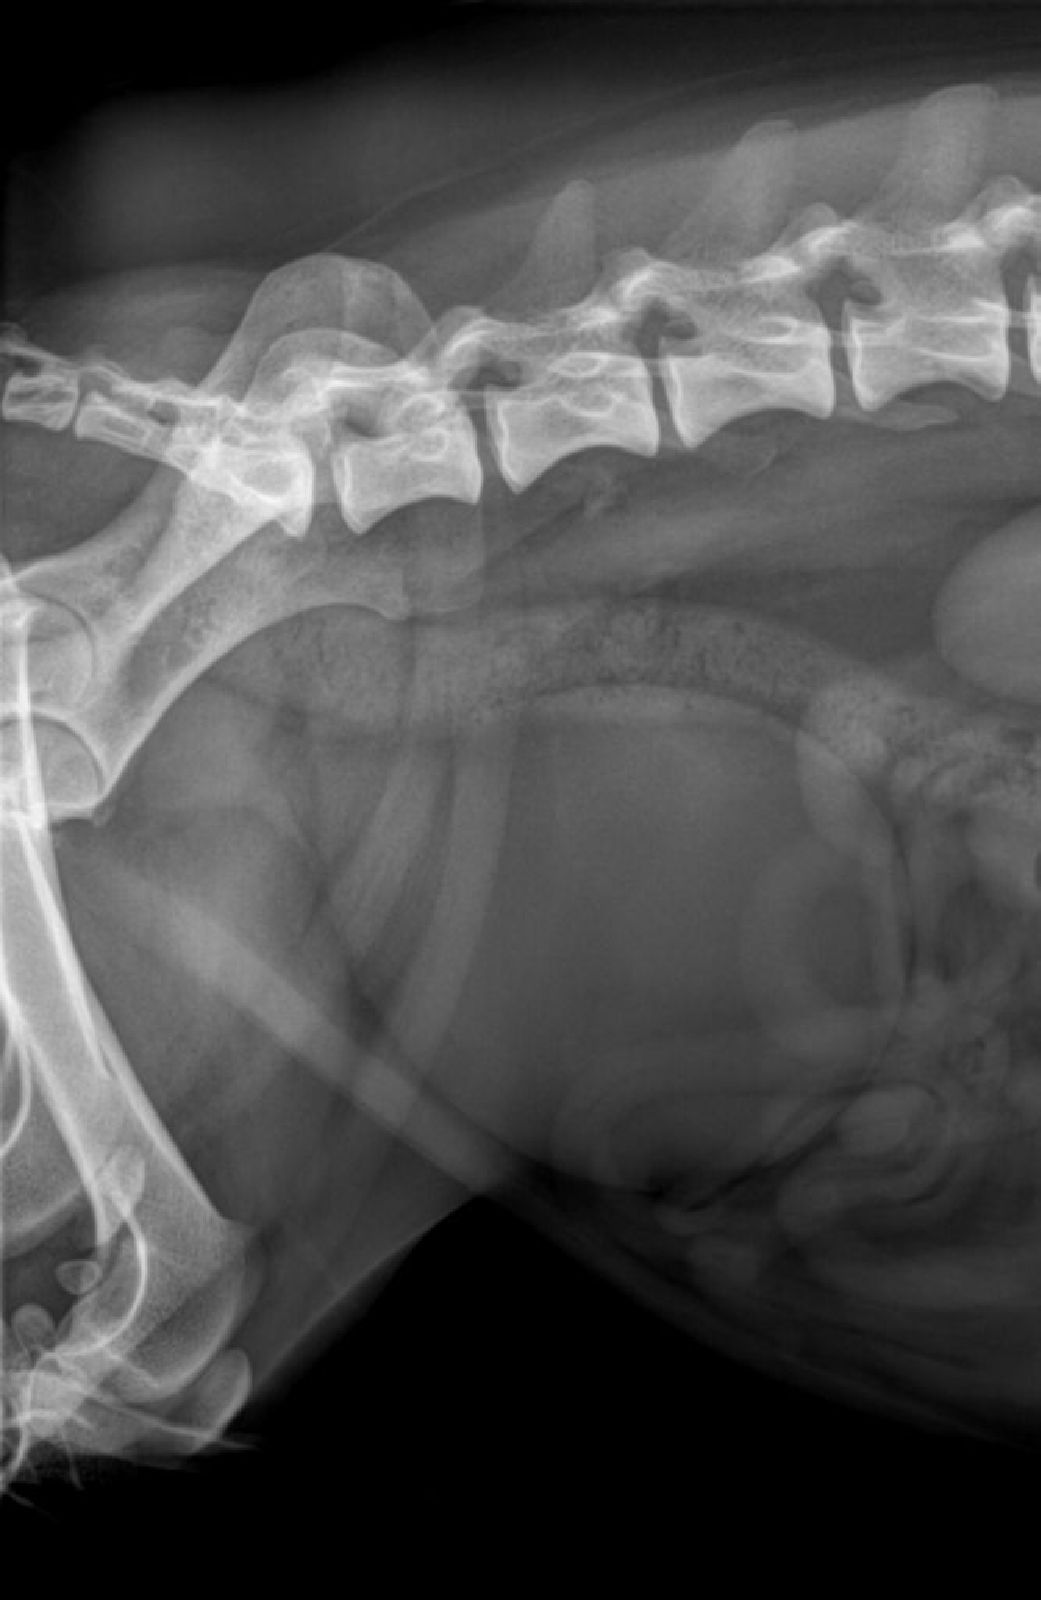
\includegraphics[scale=0.20]{3.backmatter/figures/l}} 
	\subfloat[]{\label{fig:intensity-change} 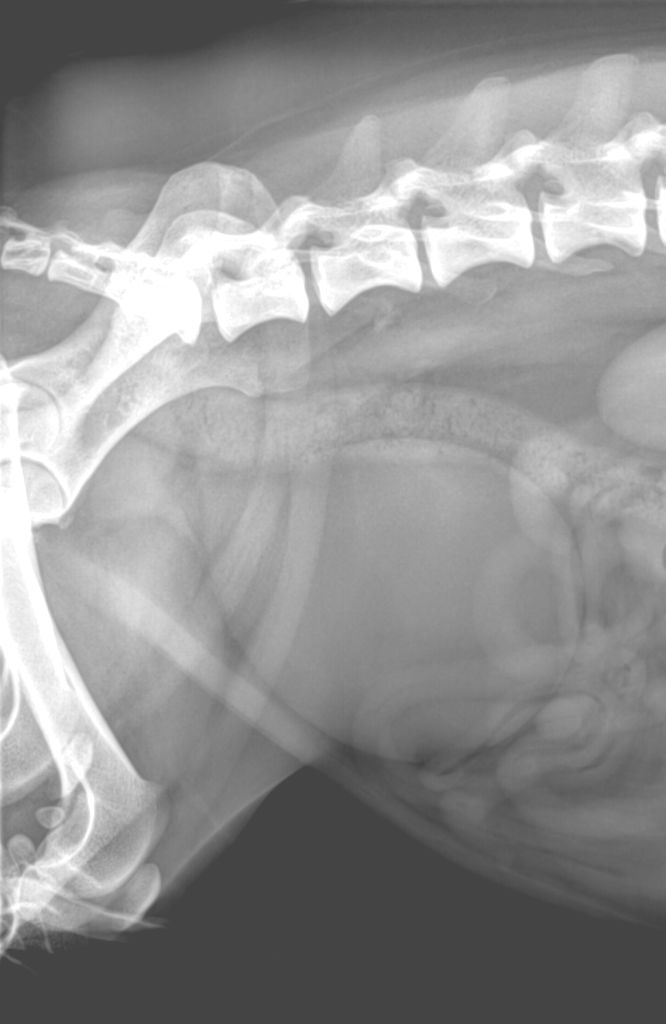
\includegraphics[scale=0.20]{3.backmatter/figures/l_br}} \quad
	\subfloat[]{\label{fig:rotation} 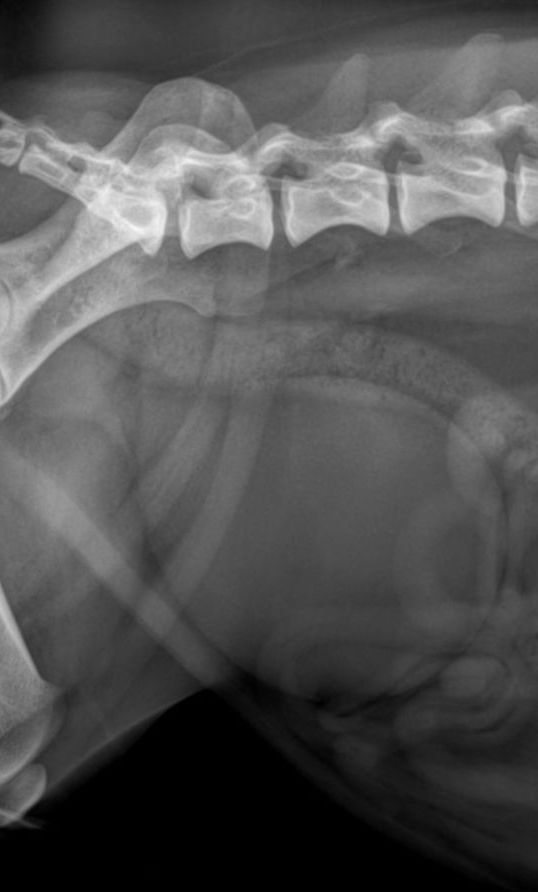
\includegraphics[scale=0.25]{3.backmatter/figures/l_rot_8}} 
	\subfloat[]{\label{fig:scaled} 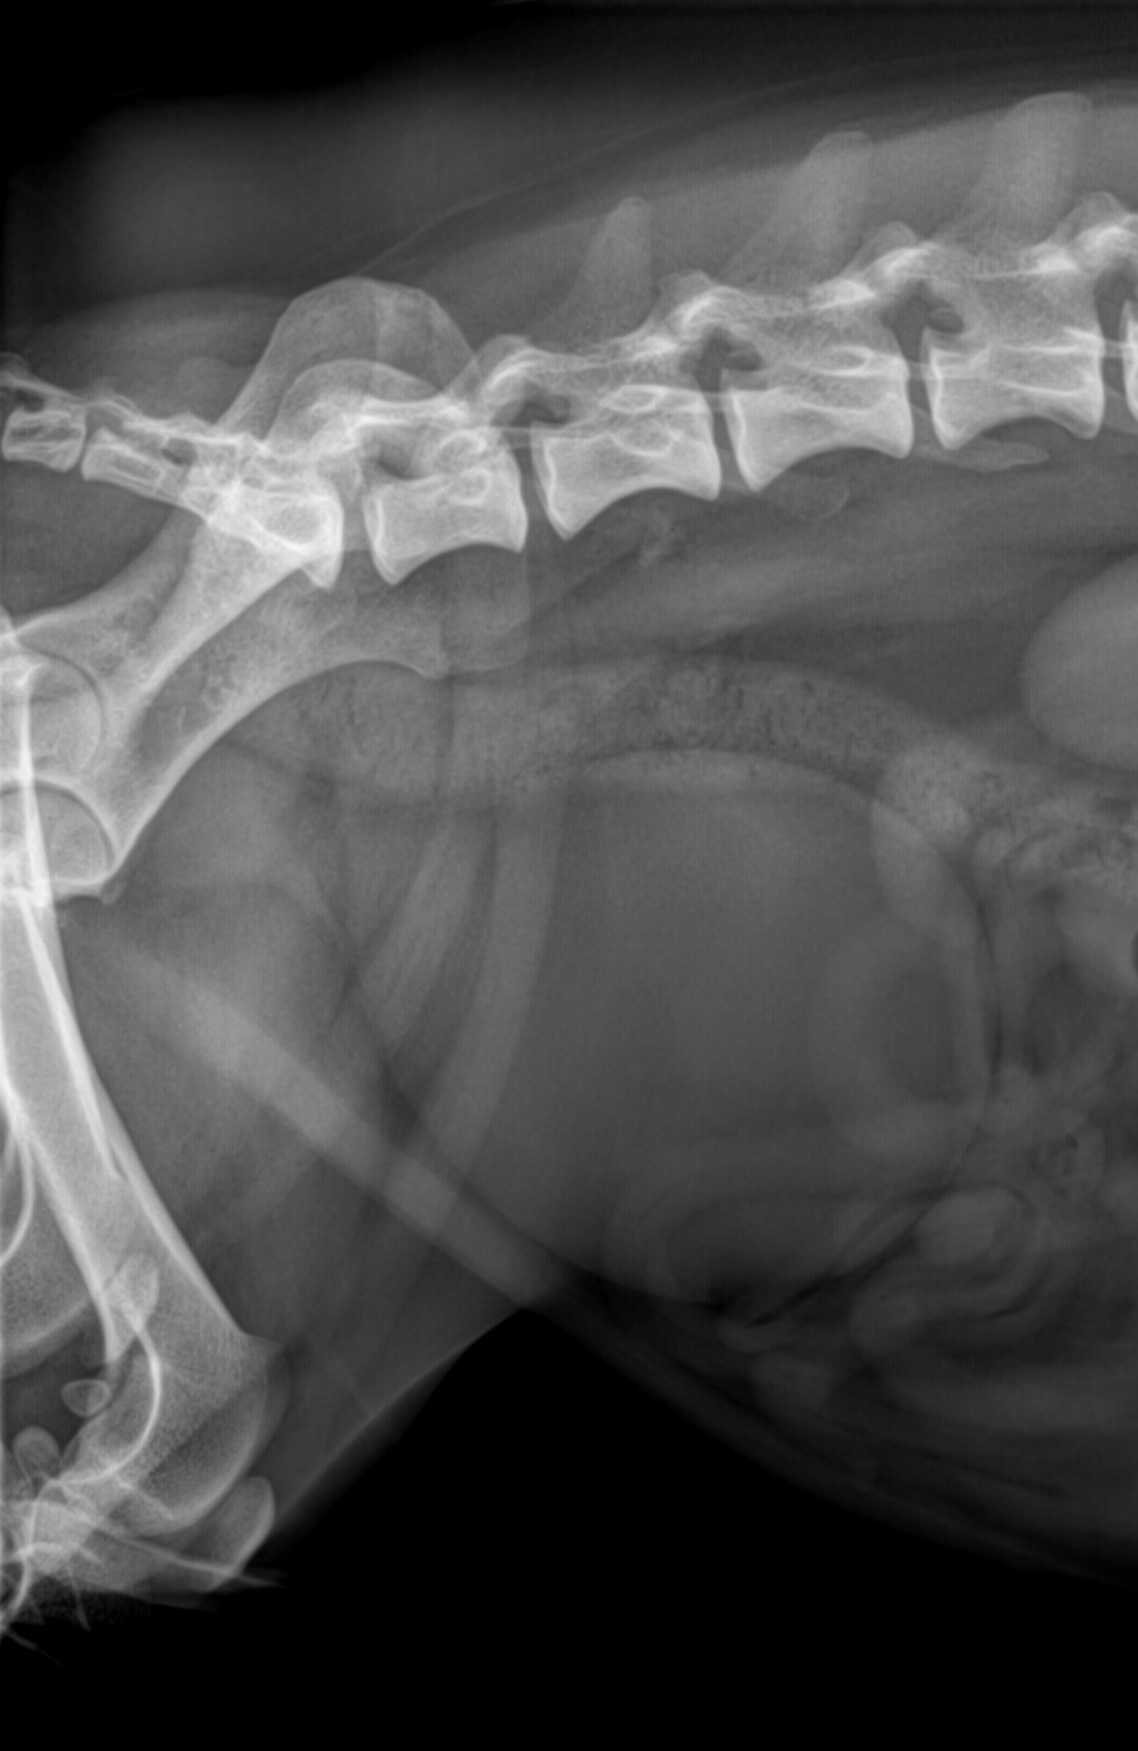
\includegraphics[scale=0.15]{3.backmatter/figures/l_large}} 	
	
	%\subfloat[]{\label{fig:intensity-rotation} 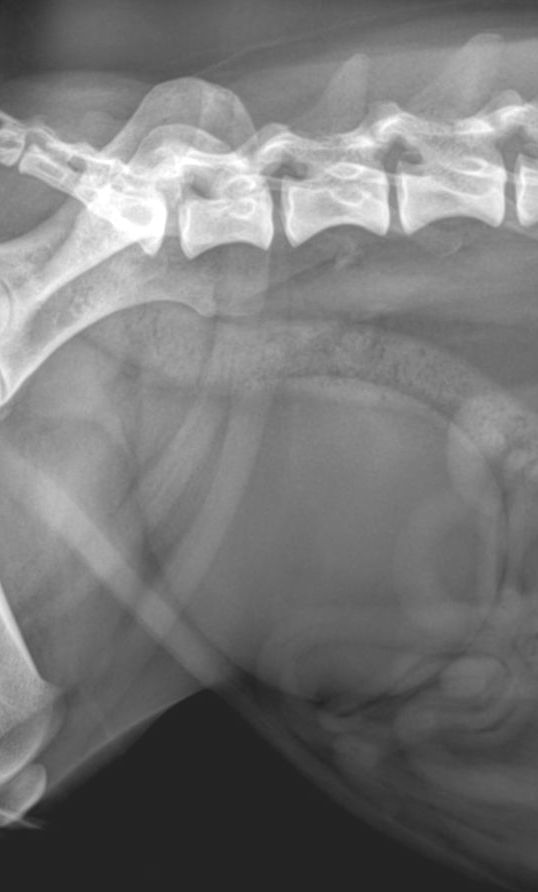
\includegraphics[scale=0.15]{3.backmatter/figures/l_br_rot}}
	%\subfloat[]{\label{fig:intensity-scaling} 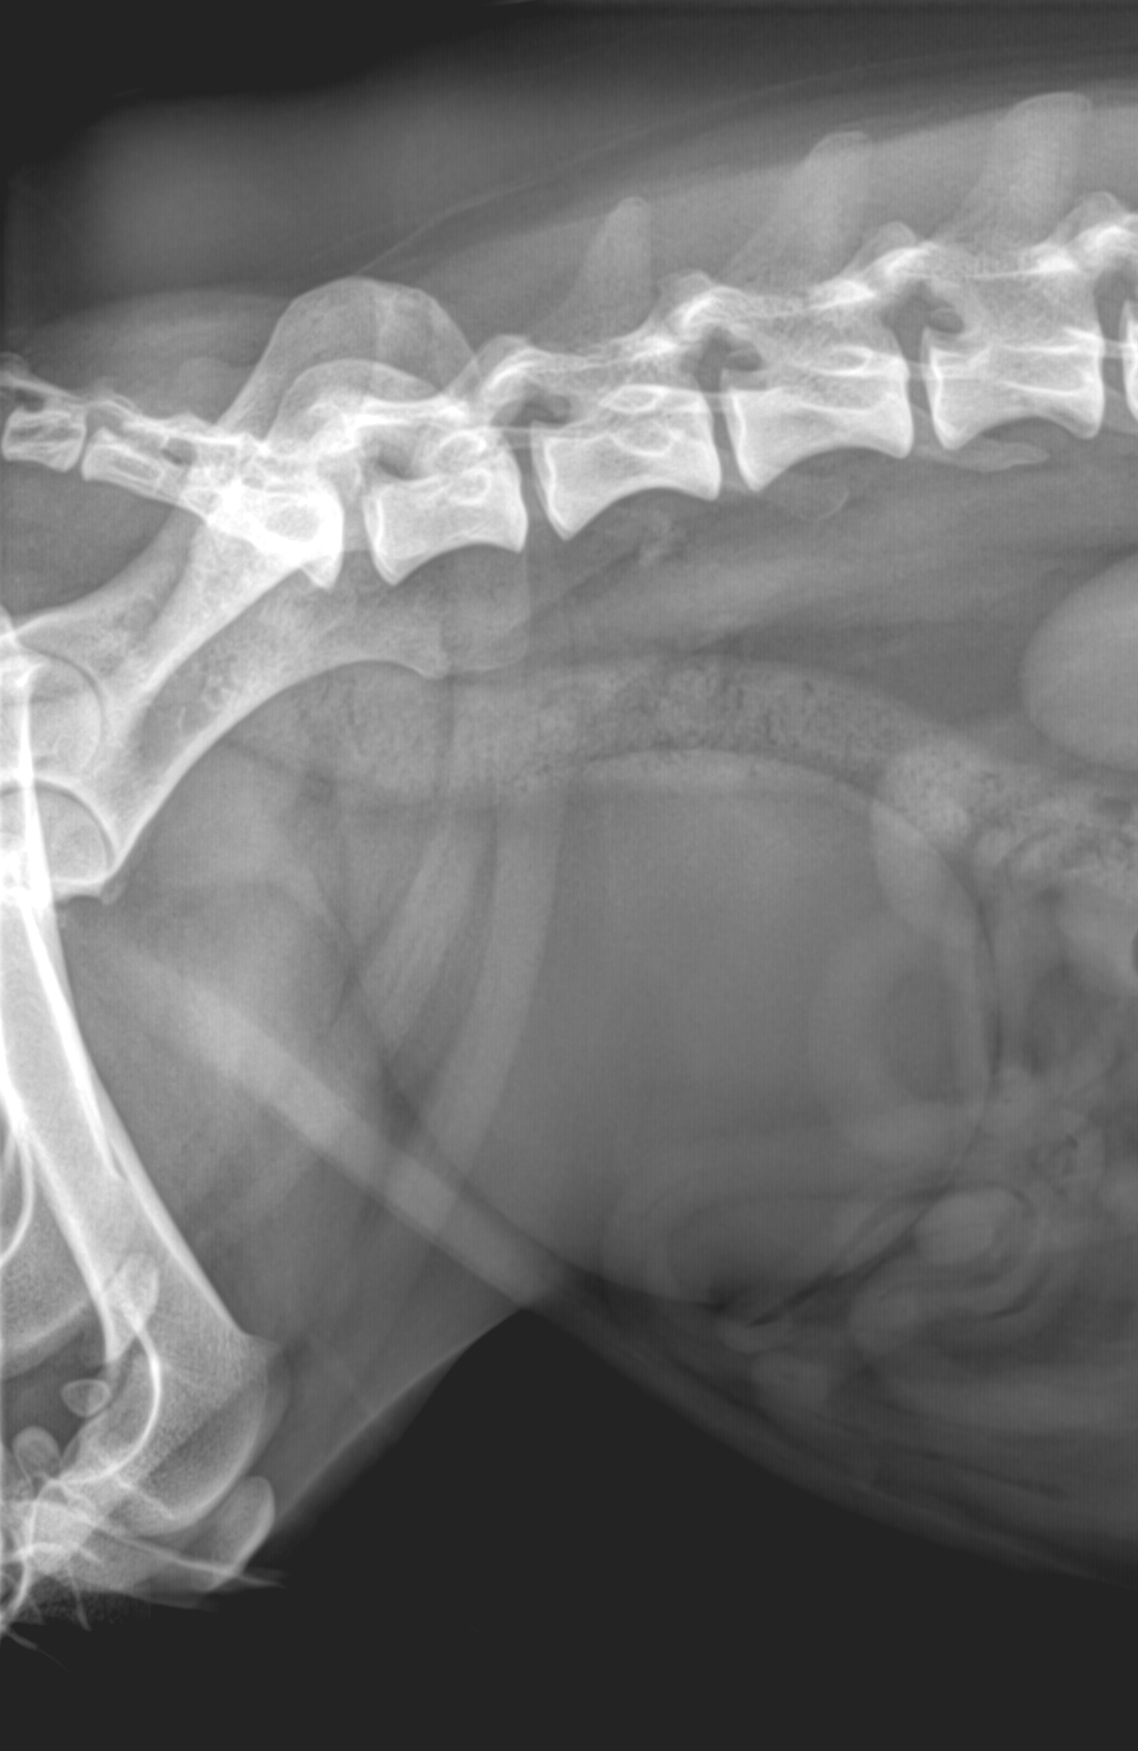
\includegraphics[scale=0.10]{3.backmatter/figures/l_large_br}} 
	%\subfloat[]{\label{fig:intensity-rotation-scaling} 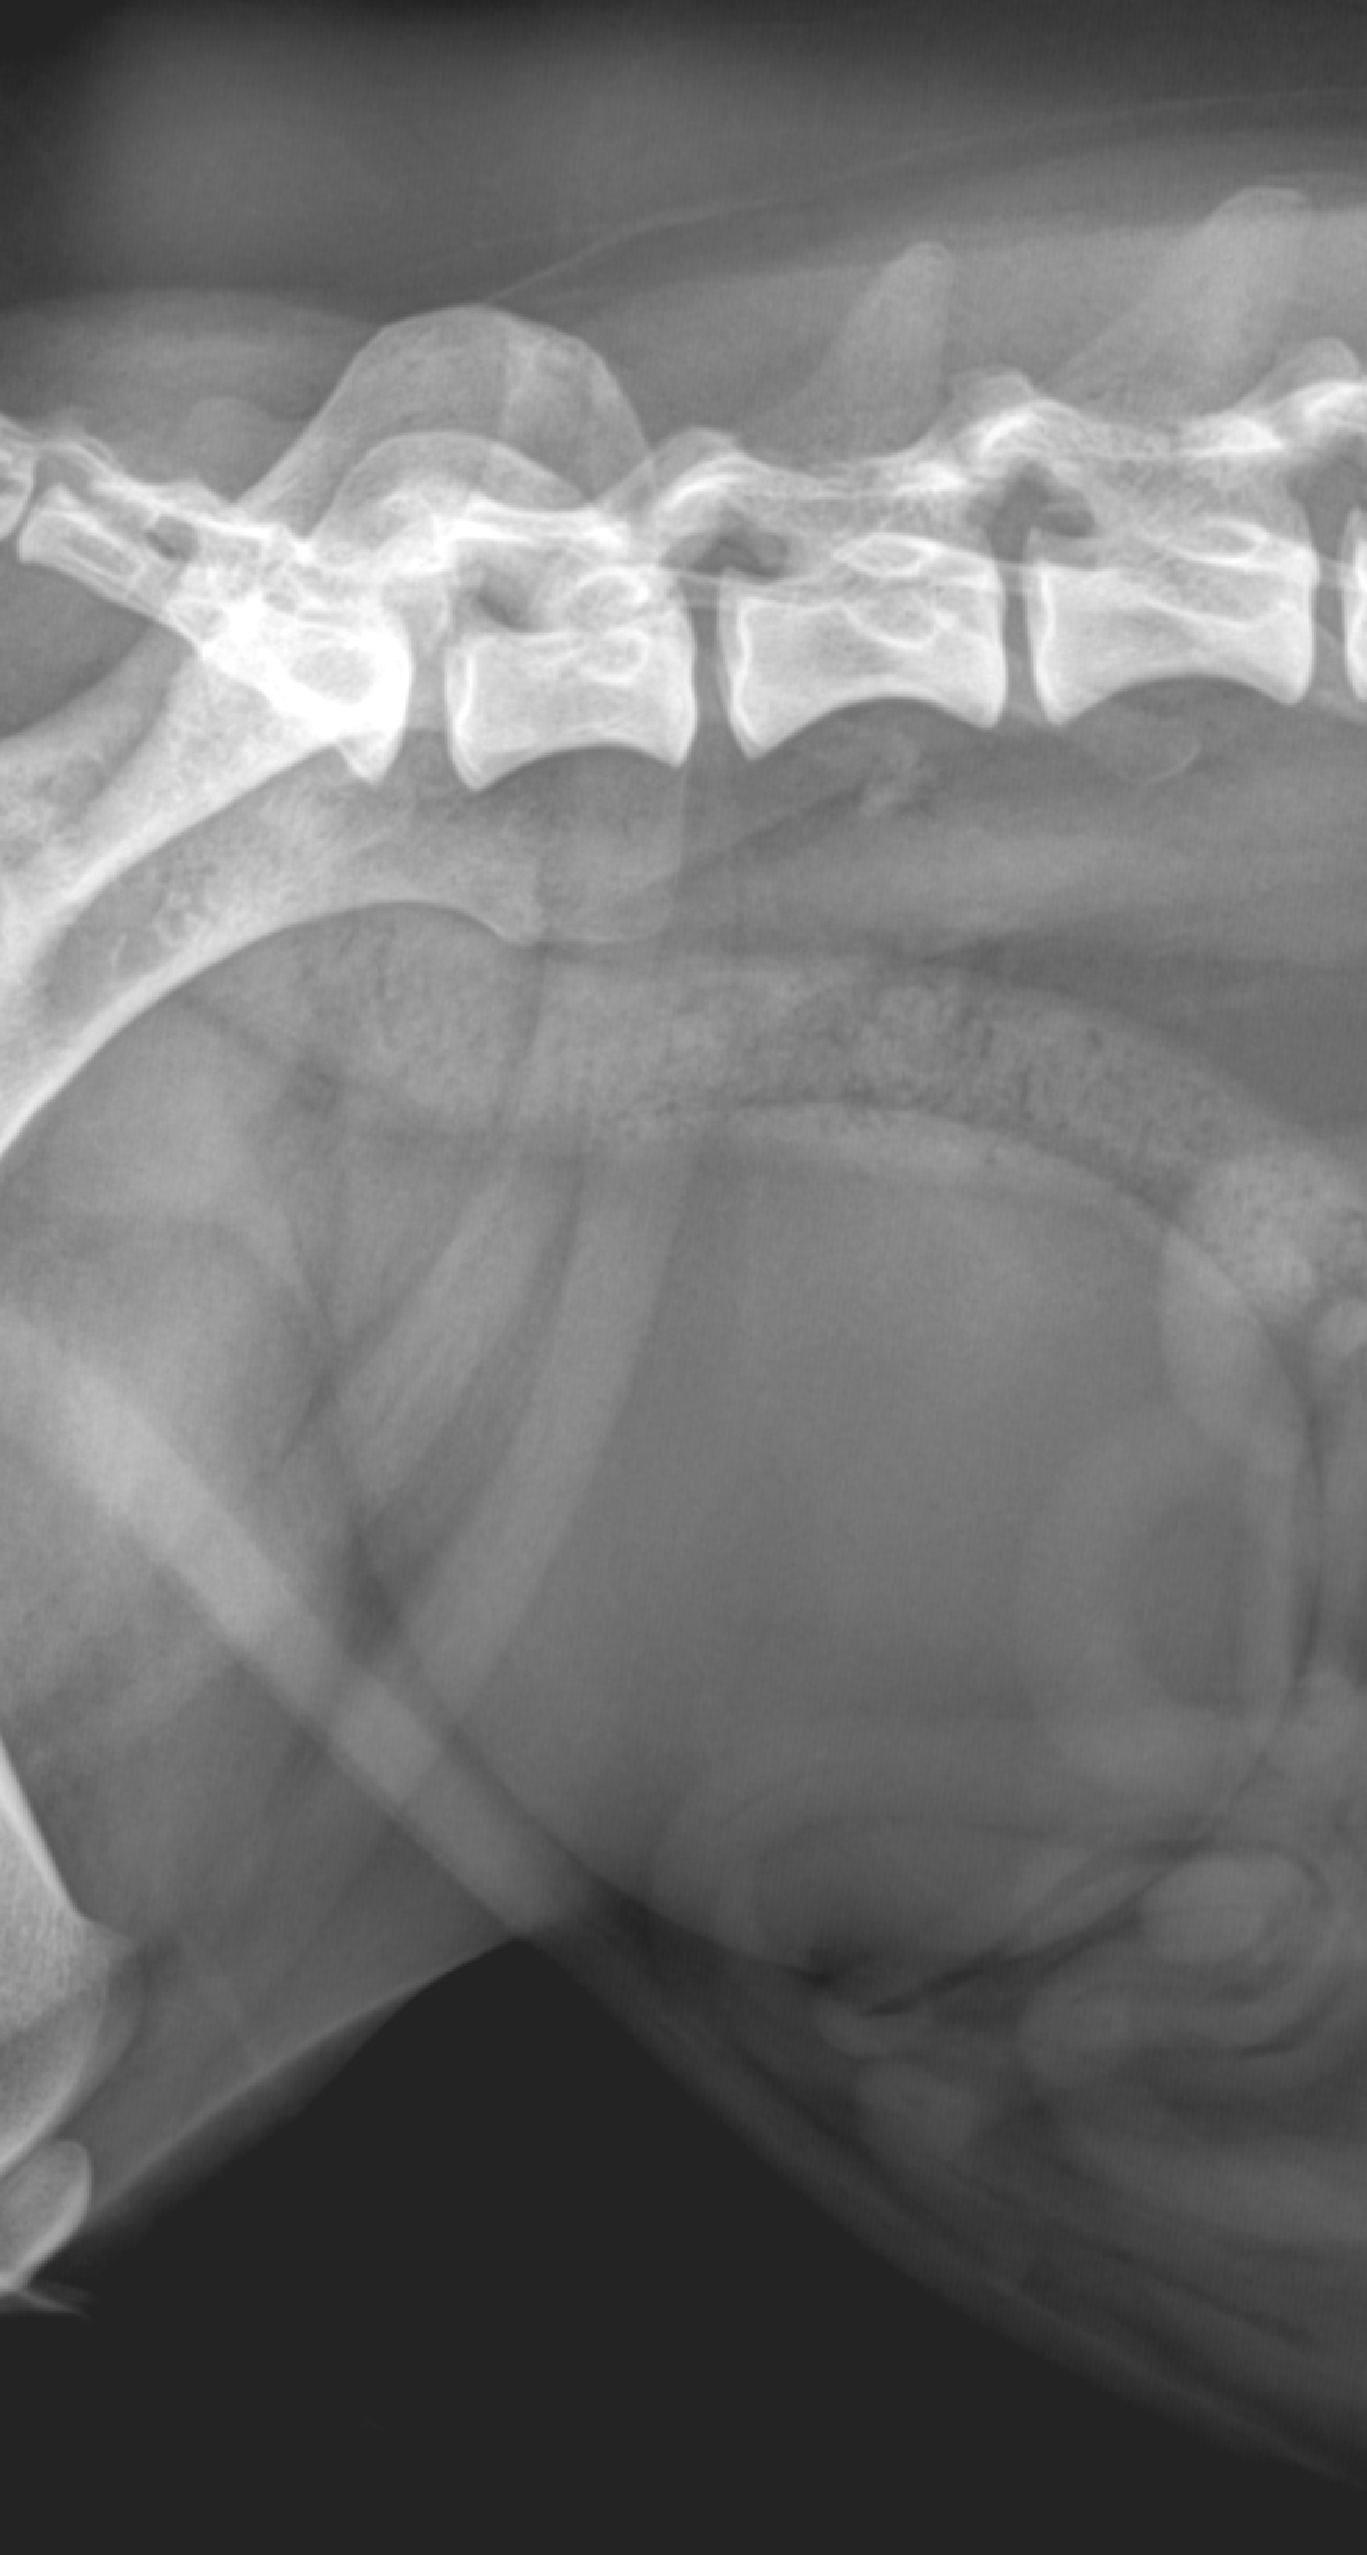
\includegraphics[scale=0.10]{3.backmatter/figures/l_large_br_rot}} 
	%\subfloat[]{\label{fig:noisy} 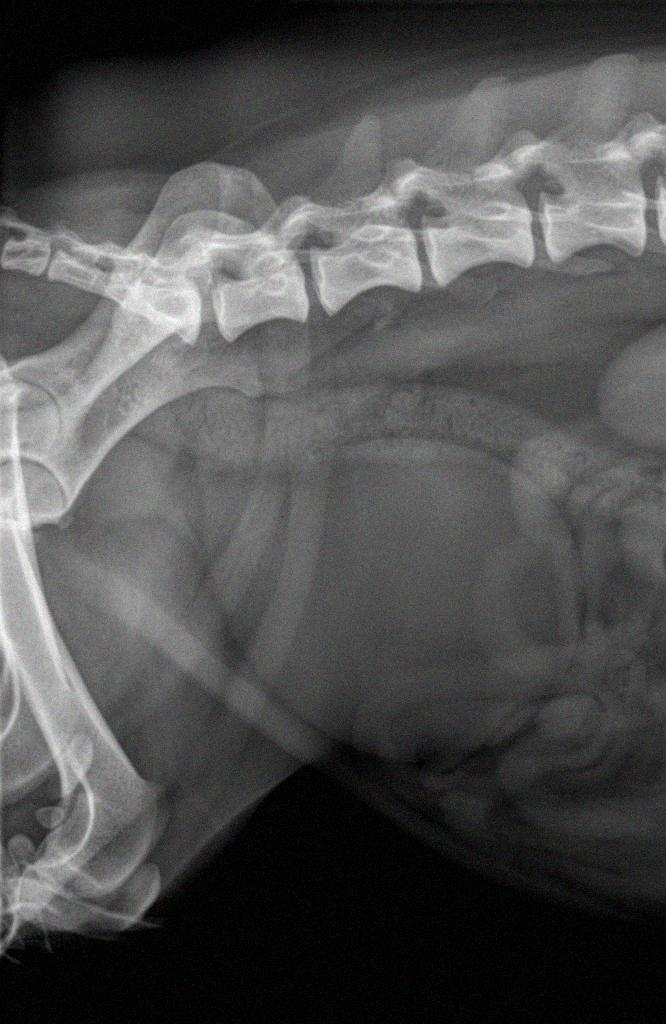
\includegraphics[scale=0.15]{3.backmatter/figures/l_noise}}  
\end{center}
\caption[Test Images to Evaluate for Feature Extractors]{Images with different intensity, orientation, scaling and noise. \subref{fig:original-image}Original Image, \subref{fig:intensity-change}Image with increased intensity, \subref{fig:rotation}Rotated image(some part is cropped to removed unused pixels) \subref{fig:scaled}Scaled image}% \subref{fig:intensity-rotation}Increase intensity \& rotation \subref{fig:intensity-scaling}Increased intensity \& scaling \subref{fig:intensity-rotation-scaling}Increased intensity, rotation \& scaling \subref{fig:noisy}Noisy image}
\end{figure}
\newpage 
\subsection{Harris Corner Detector}
\begin{figure}[H]%
\begin{center}
	\subfloat[]{\label{fig:original-image}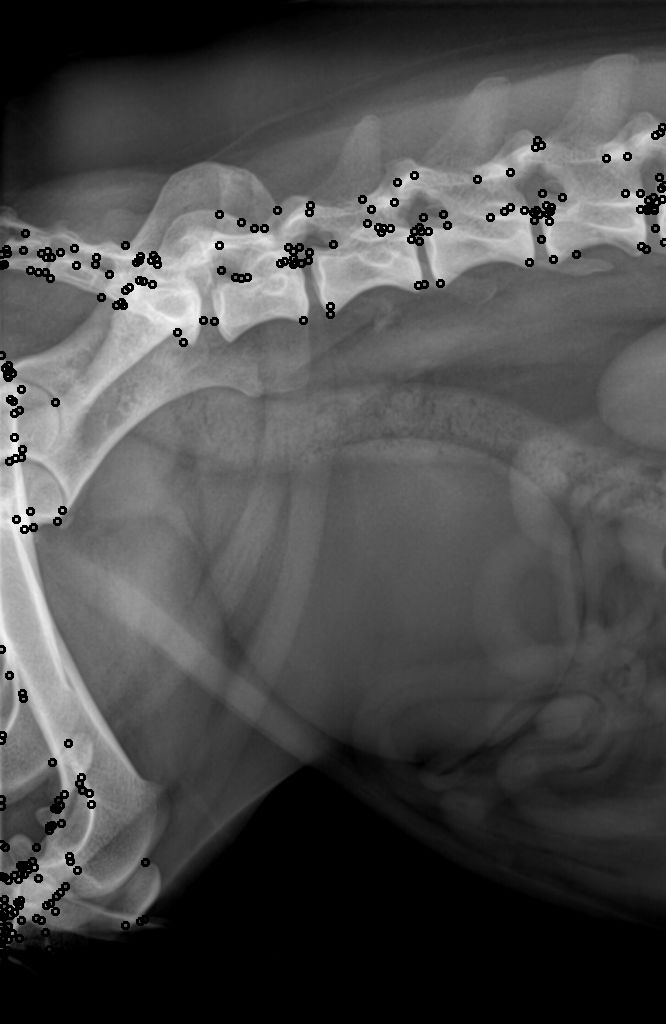
\includegraphics[scale=0.20]{3.backmatter/figures/harris/l}} 
	\subfloat[]{\label{fig:intensity-change} 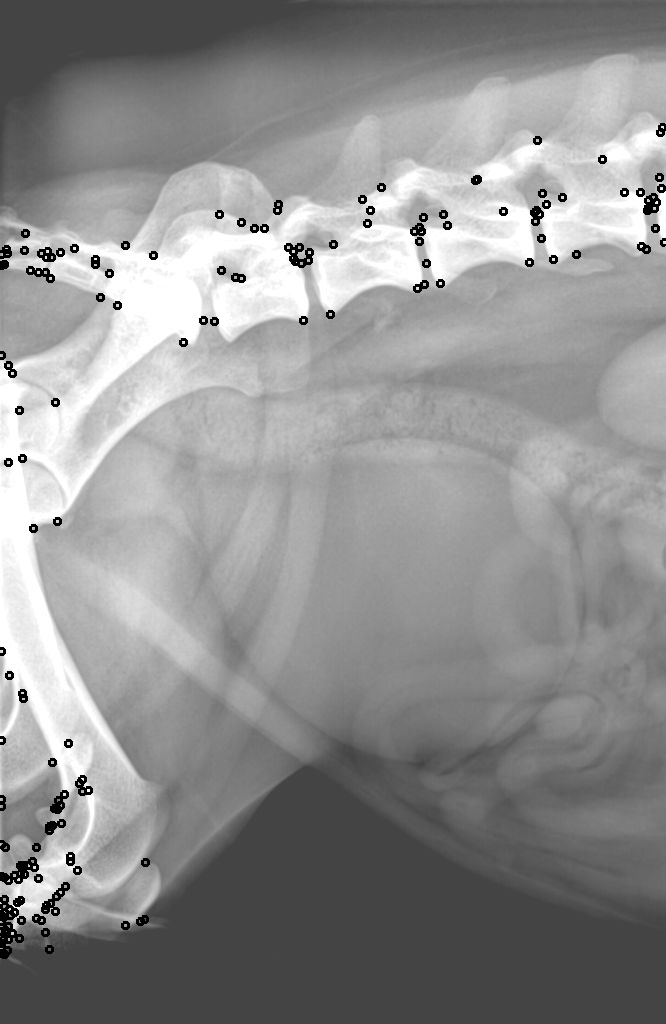
\includegraphics[scale=0.20]{3.backmatter/figures/harris/l_br}} \quad
	\subfloat[]{\label{fig:rotation} 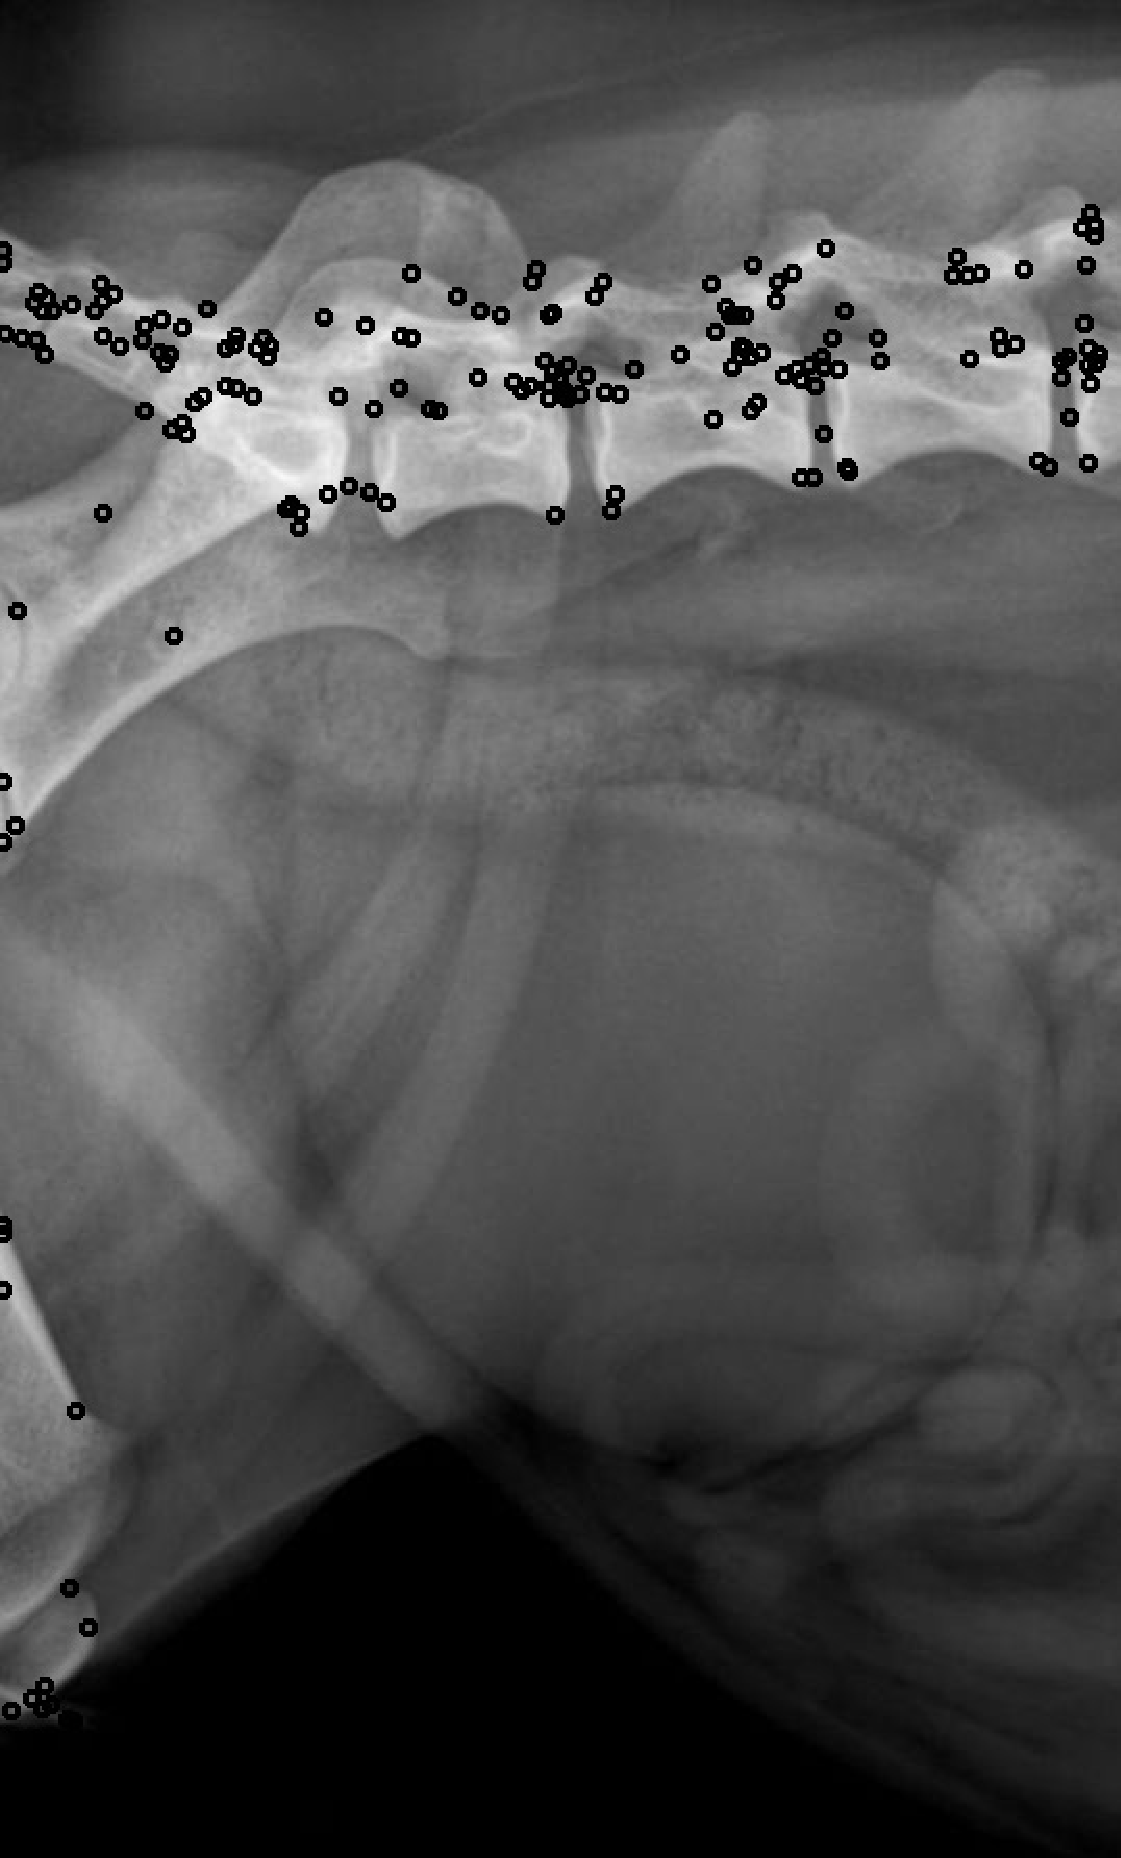
\includegraphics[scale=0.25]{3.backmatter/figures/harris/l_rot_8}}	
	\subfloat[]{\label{fig:scaled} 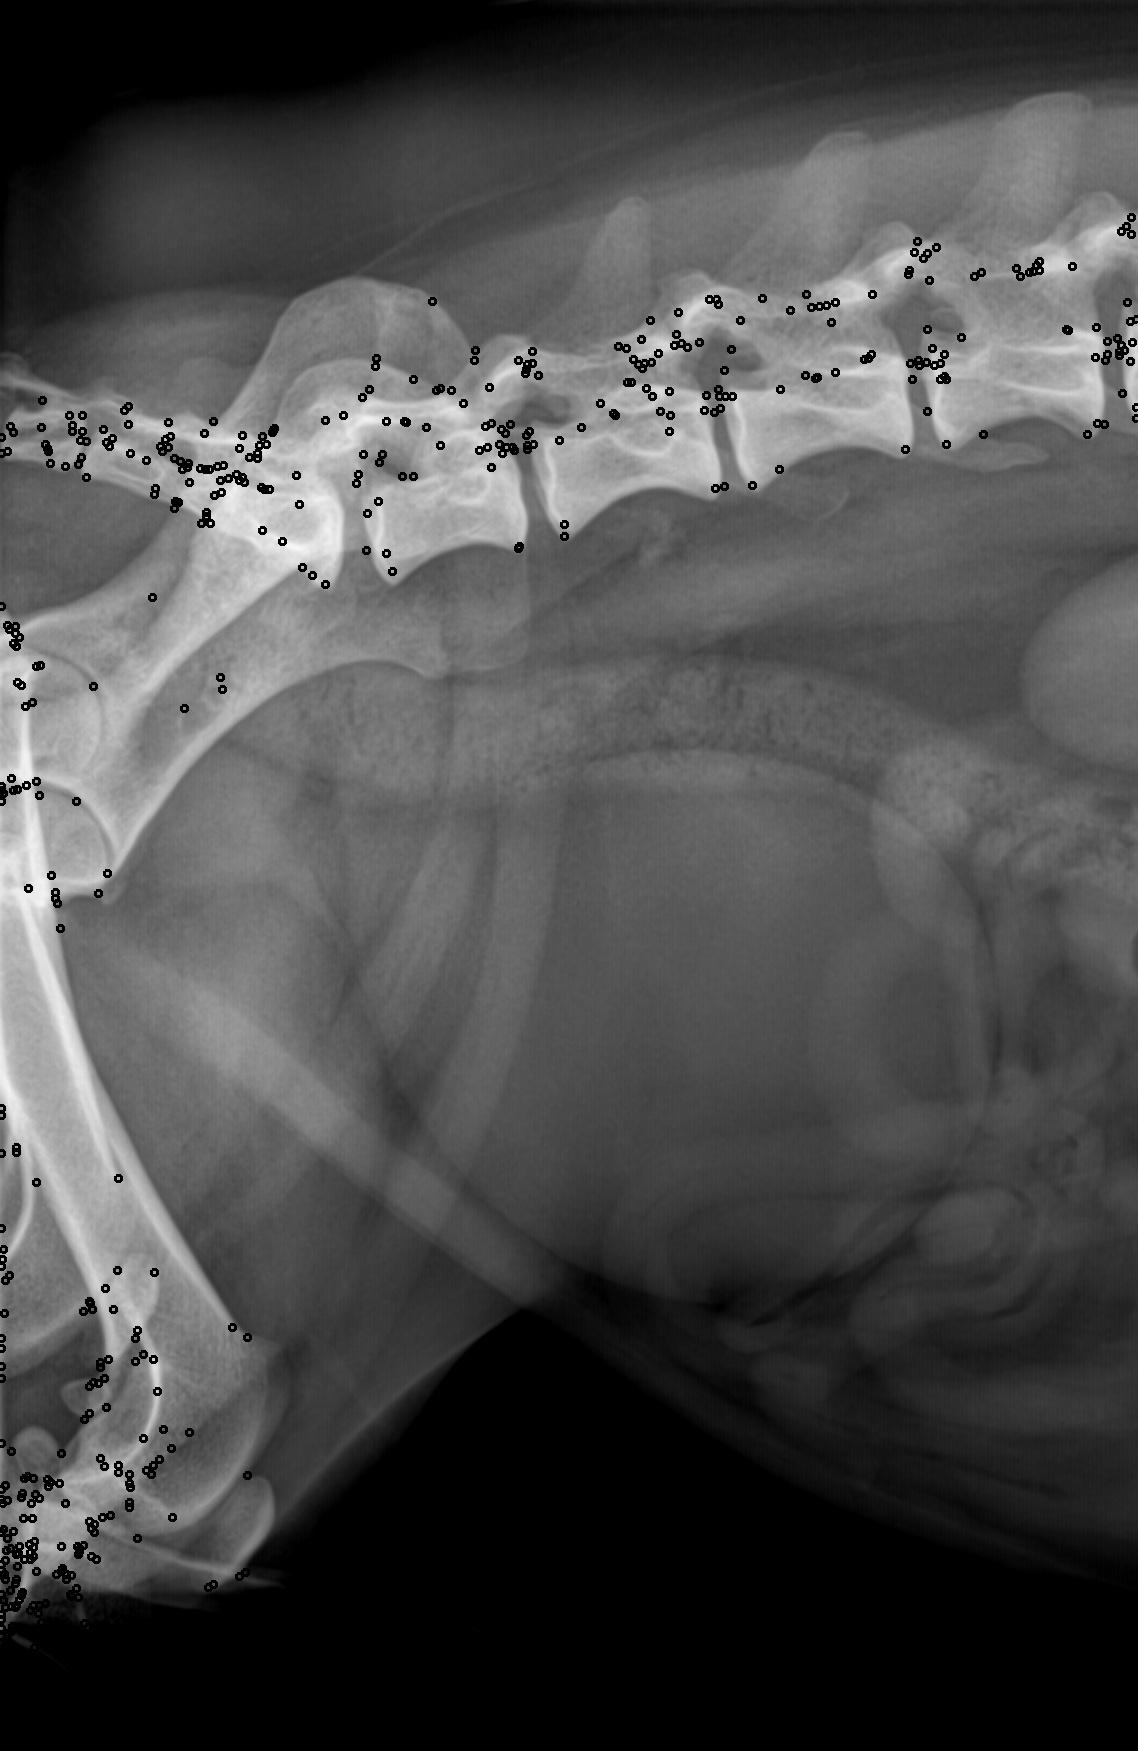
\includegraphics[scale=0.15]{3.backmatter/figures/harris/l_large}} 	
	%\subfloat[]{\label{fig:intensity-rotation} 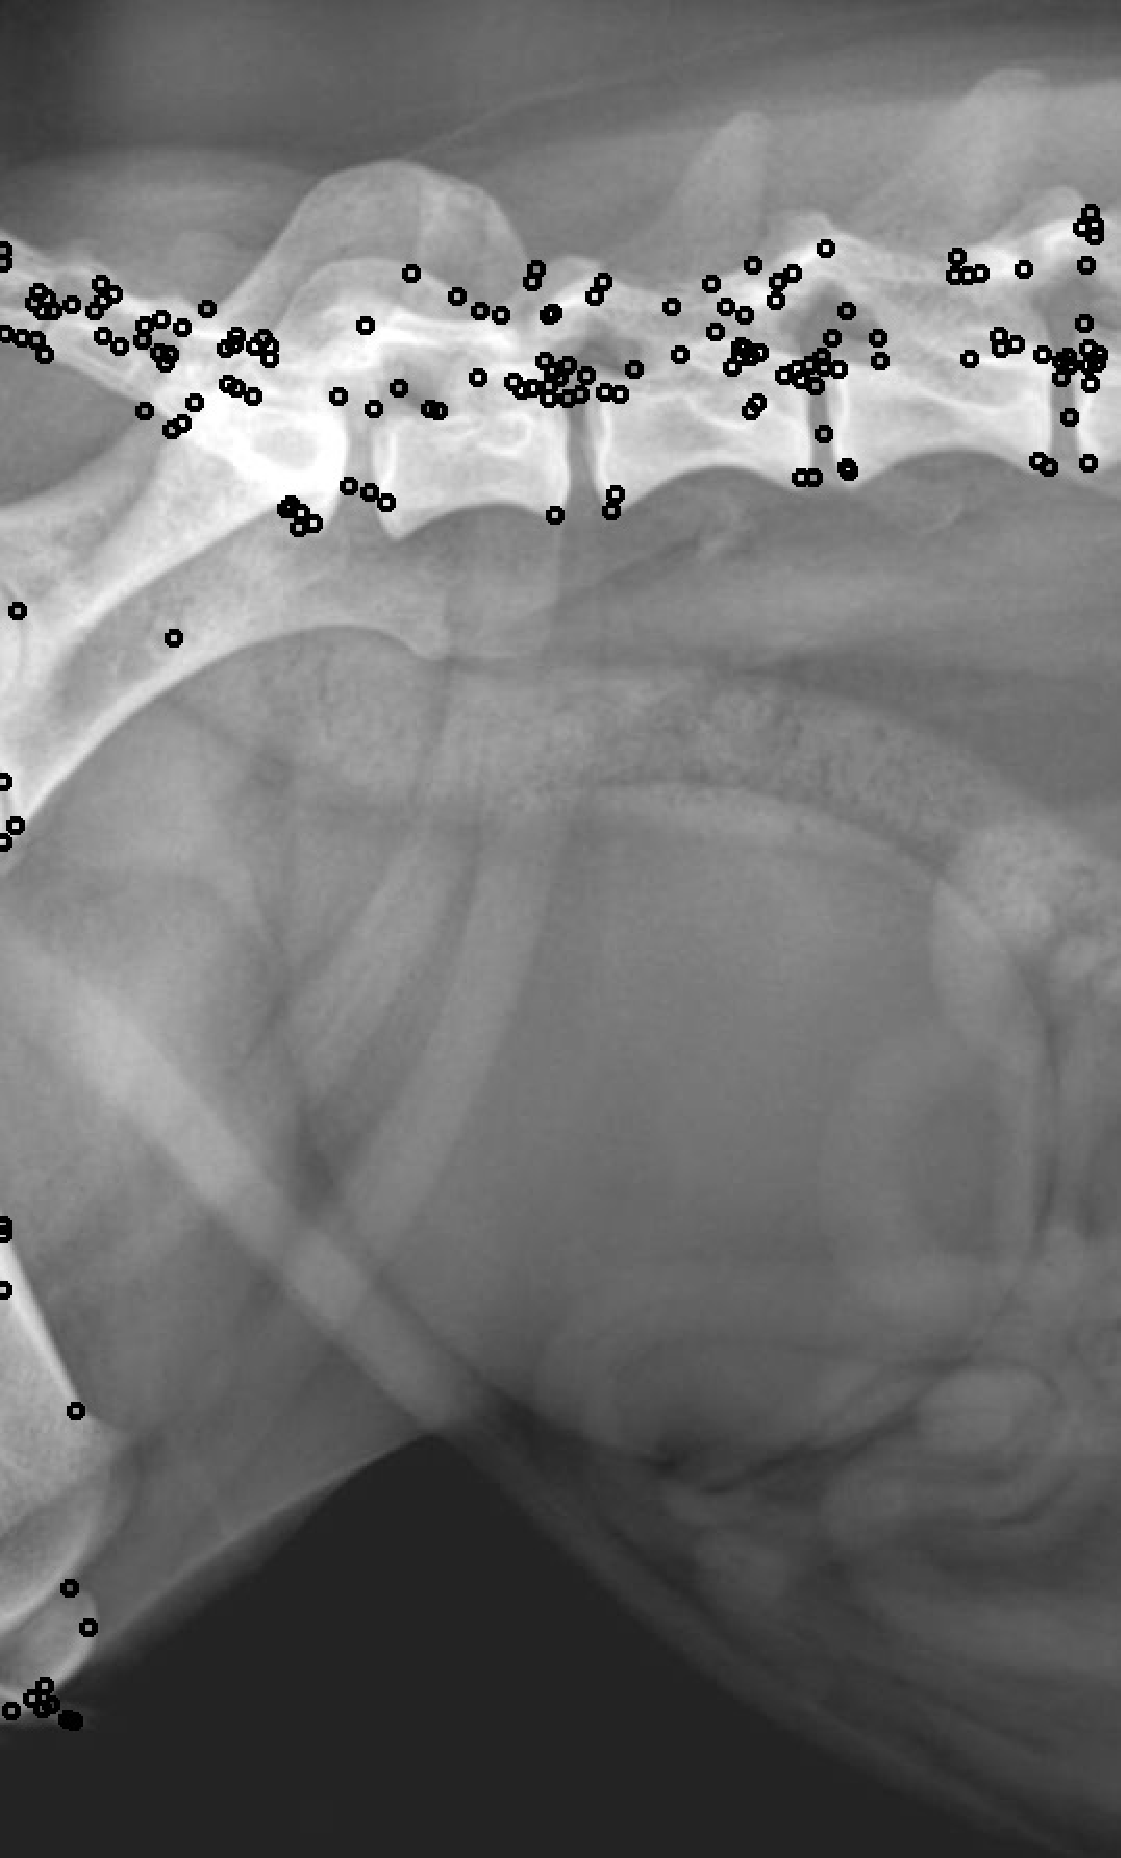
\includegraphics[scale=0.15]{3.backmatter/figures/harris/l_br_rot}}
	%\subfloat[]{\label{fig:intensity-scaling} 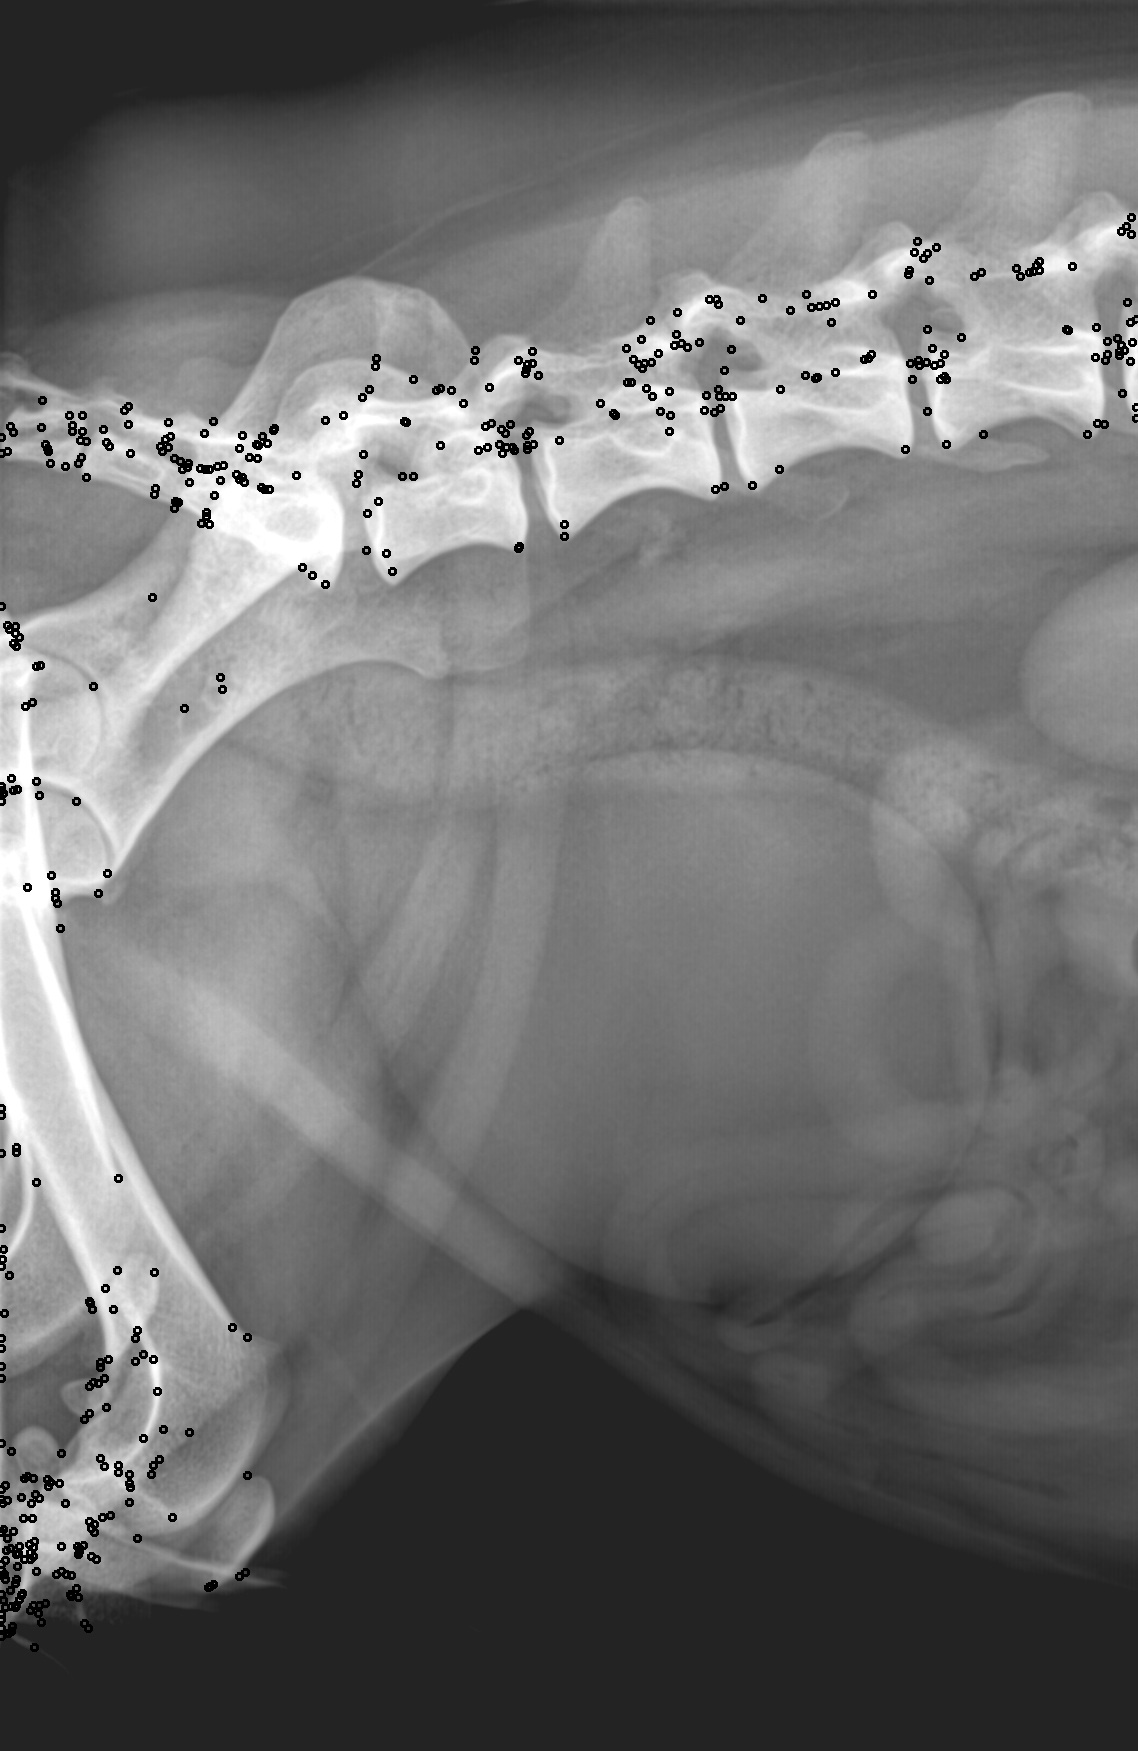
\includegraphics[scale=0.10]{3.backmatter/figures/harris/l_large_br}} 
	%\subfloat[]{\label{fig:intensity-rotation-scaling} 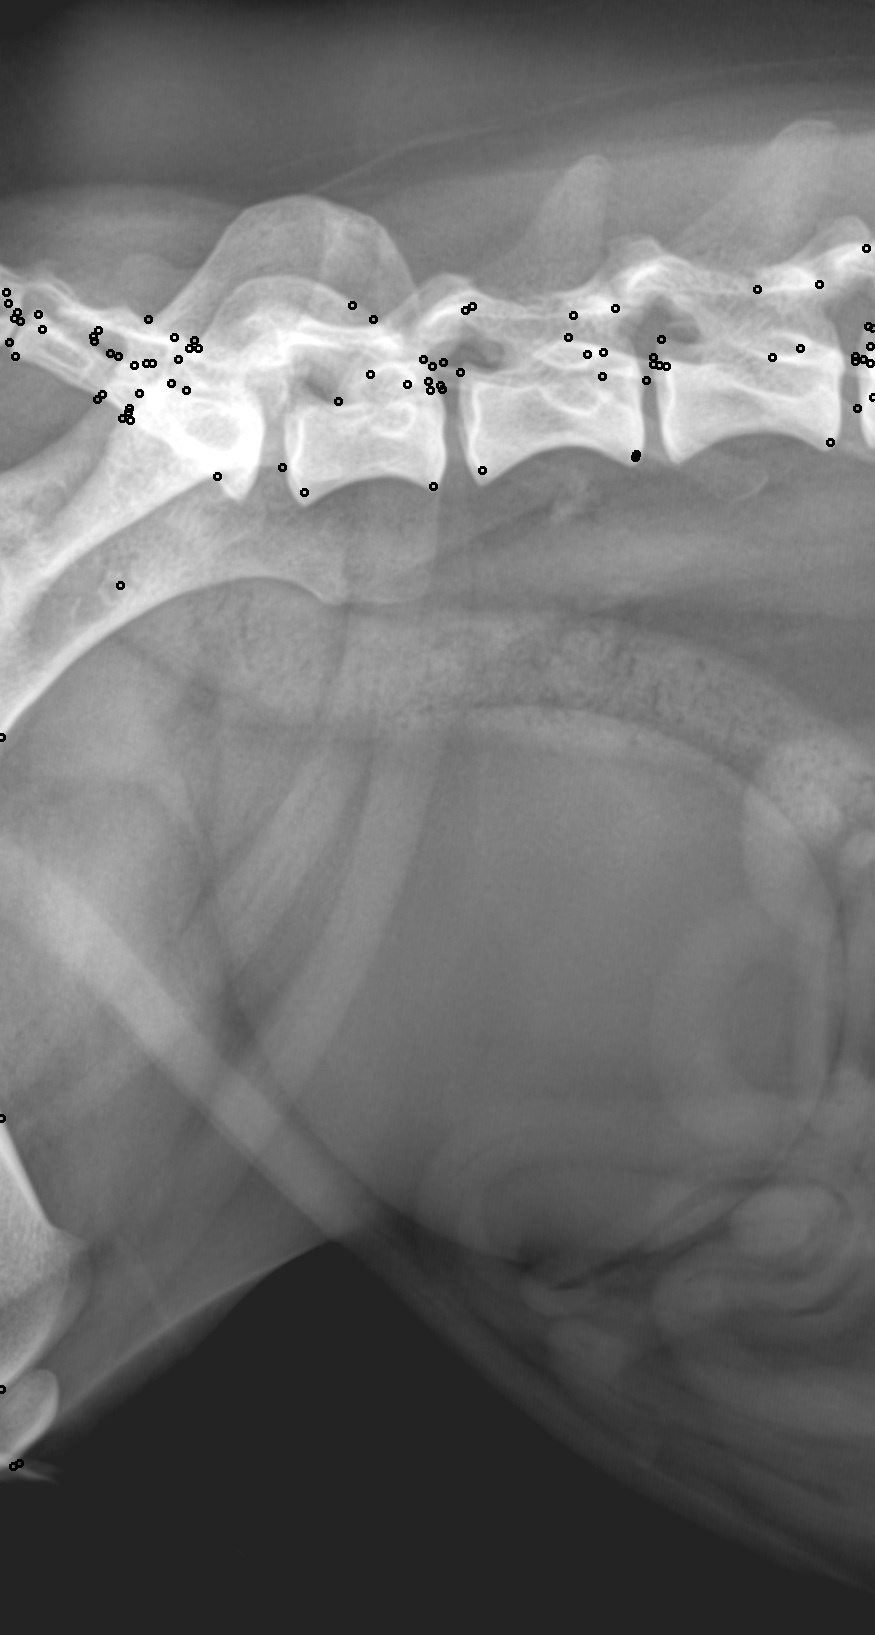
\includegraphics[scale=0.10]{3.backmatter/figures/harris/l_large_br_rot}} 
	%\subfloat[]{\label{fig:noisy} 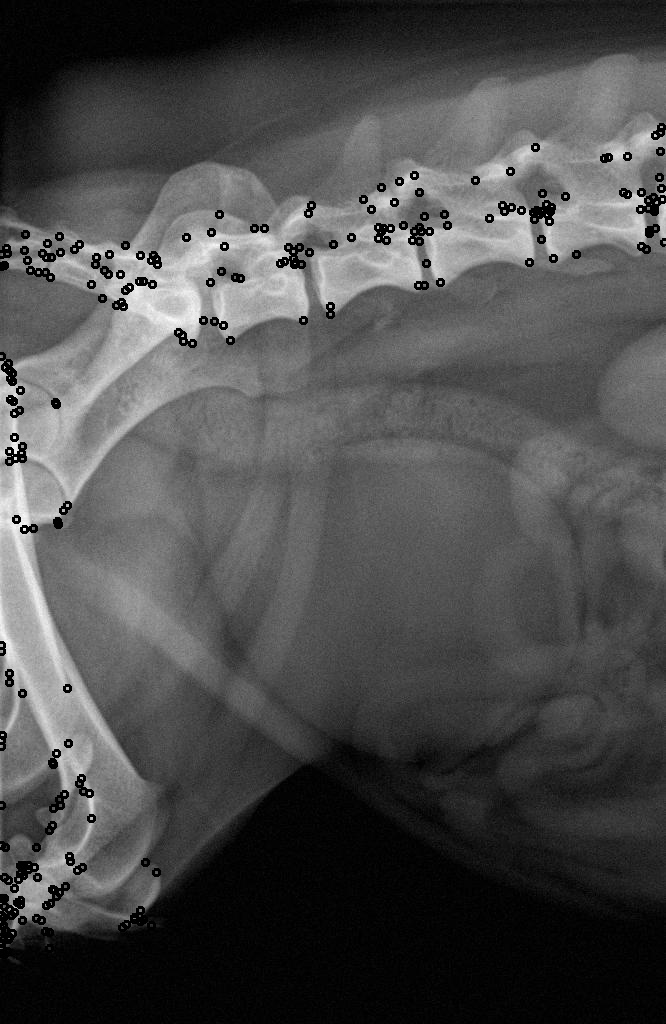
\includegraphics[scale=0.15]{3.backmatter/figures/harris/l_noise}}  
\end{center}
\caption[Result of Harris Corner Detector]{Result of Harris Corner Detector. \subref{fig:original-image}Original Image, \subref{fig:intensity-change}Image with increased intensity, \subref{fig:rotation}Rotated image(some part is cropped to remove unused pixels) \subref{fig:scaled}Scaled image}% \subref{fig:intensity-rotation}Increase intensity \& rotation \subref{fig:intensity-scaling}Increased intensity \& scaling \subref{fig:intensity-rotation-scaling}Increased intensity, rotation \& scaling \subref{fig:noisy}Noisy image}
\end{figure}

\subsection{SIFT}
\begin{figure}[H]%
\begin{center}
	\subfloat[]{\label{fig:original-image}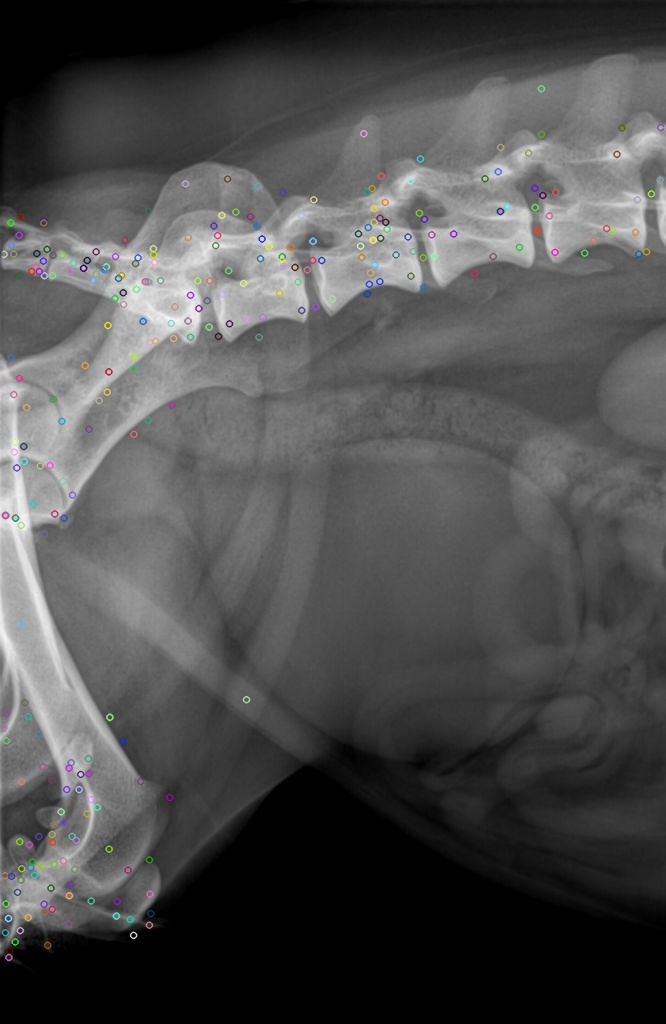
\includegraphics[scale=0.20]{3.backmatter/figures/sift/l}} 
	\subfloat[]{\label{fig:intensity-change} 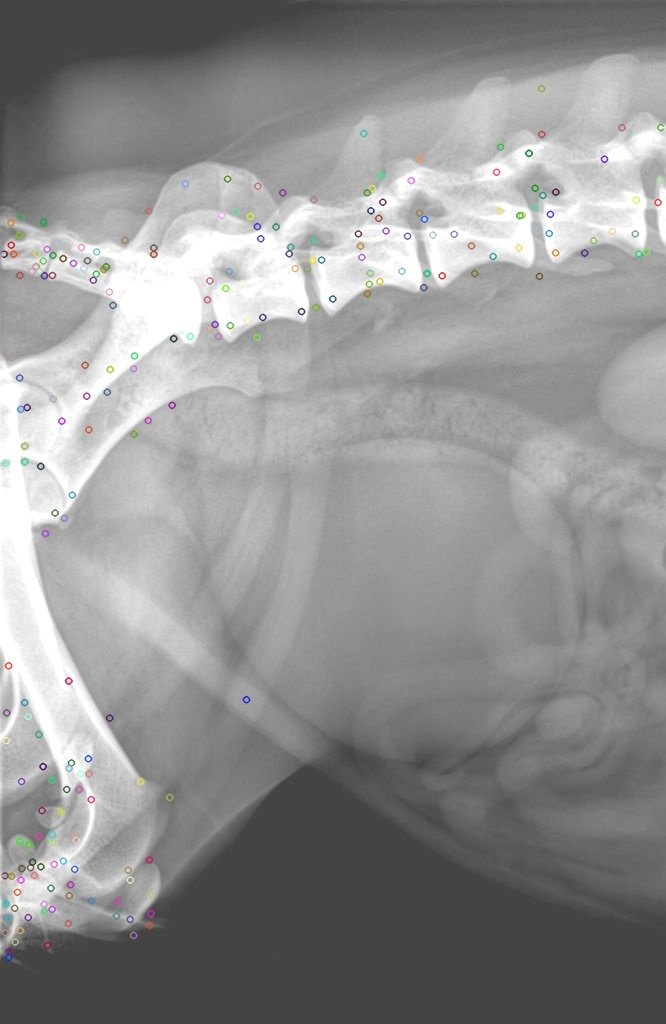
\includegraphics[scale=0.20]{3.backmatter/figures/sift/l_br}} \quad
	\subfloat[]{\label{fig:rotation} 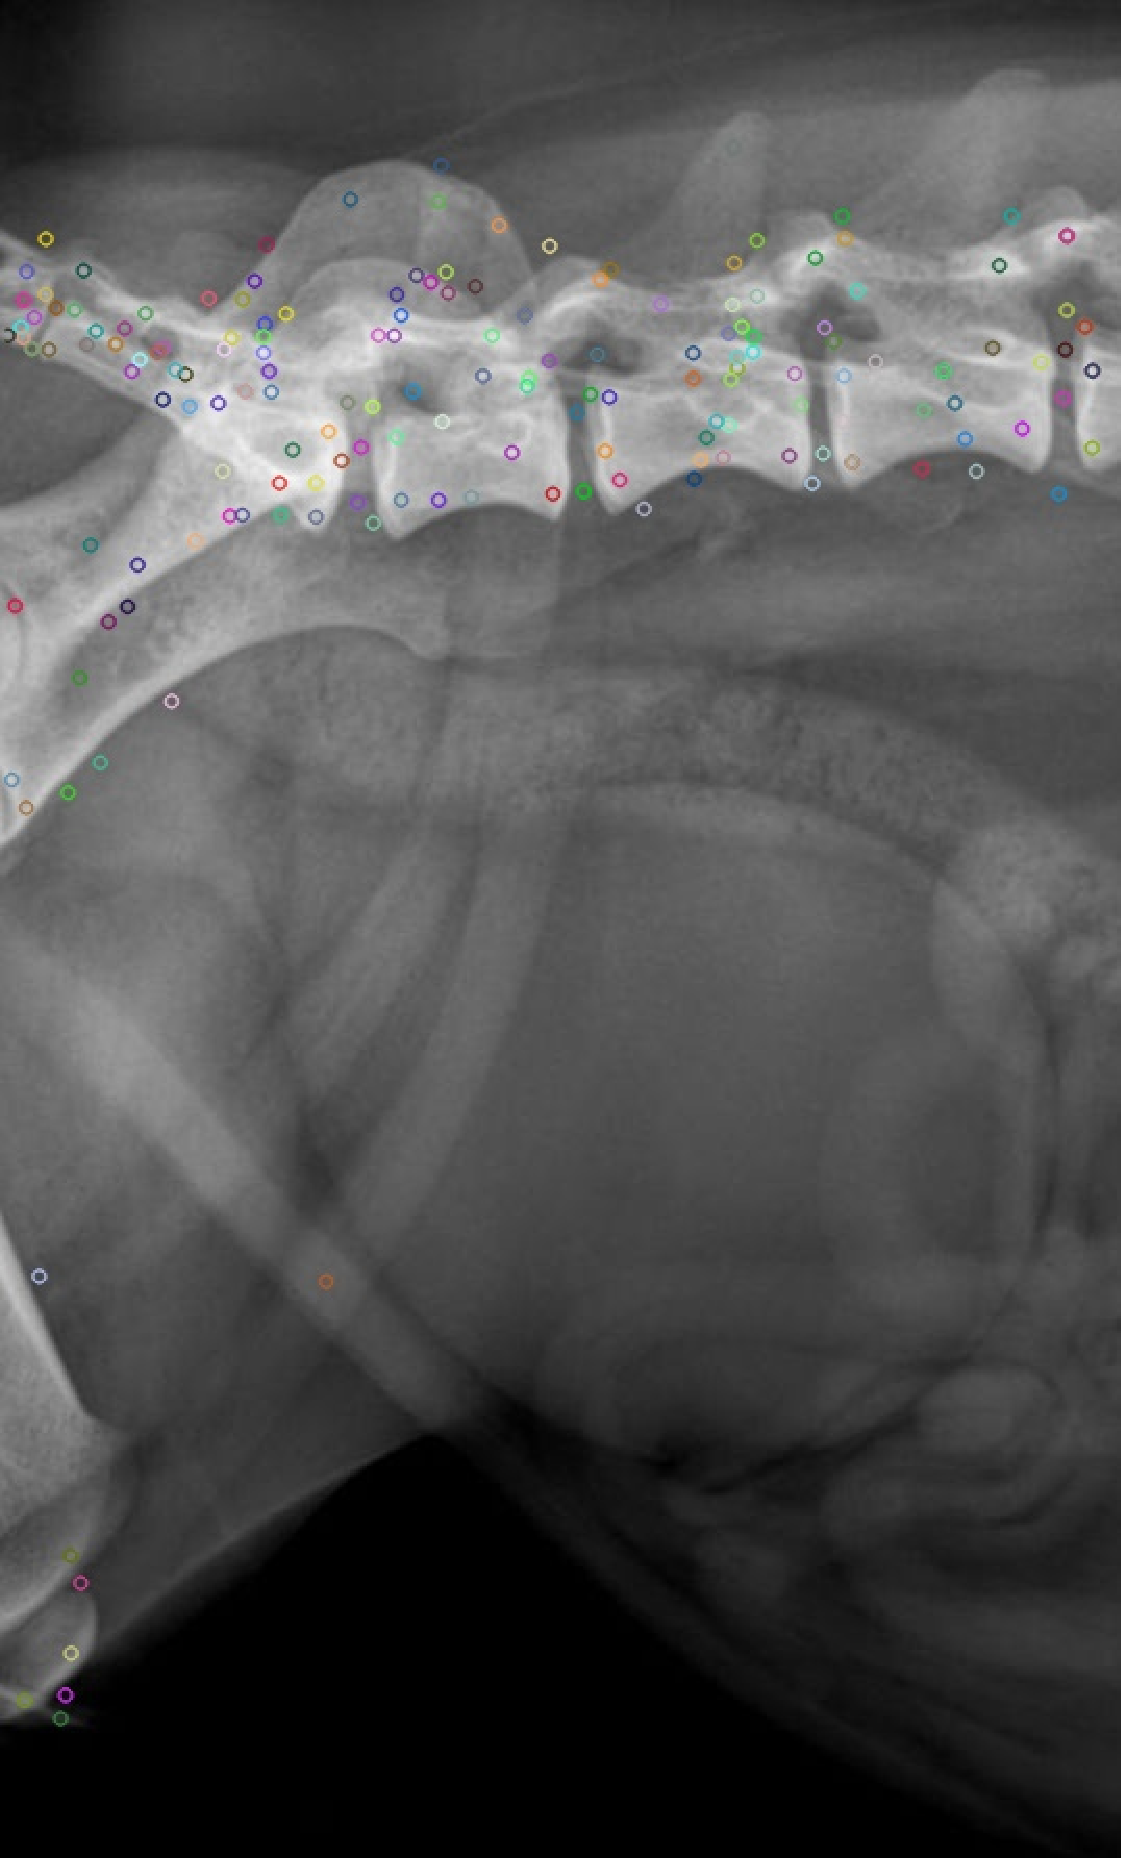
\includegraphics[scale=0.25]{3.backmatter/figures/sift/l_rot_8}}	
	\subfloat[]{\label{fig:scaled} 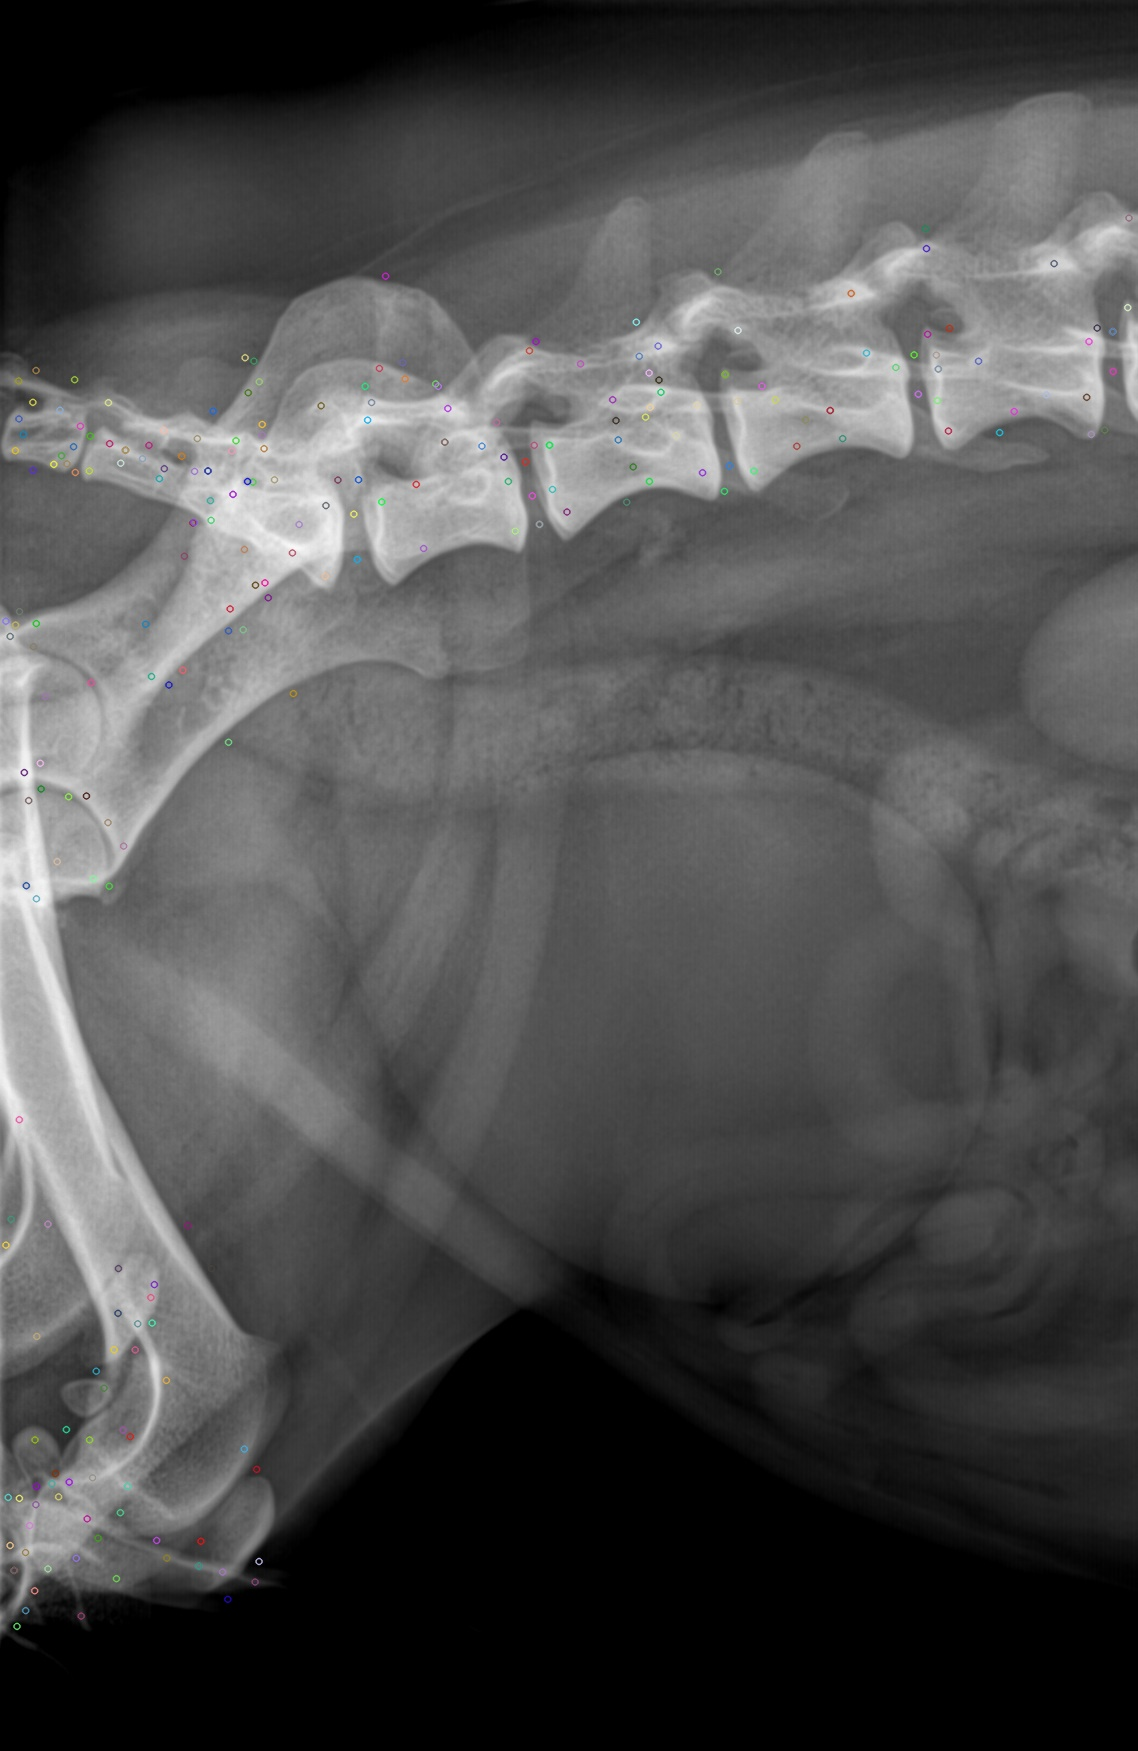
\includegraphics[scale=0.15]{3.backmatter/figures/sift/l_large}} 	
	%\subfloat[]{\label{fig:intensity-rotation} 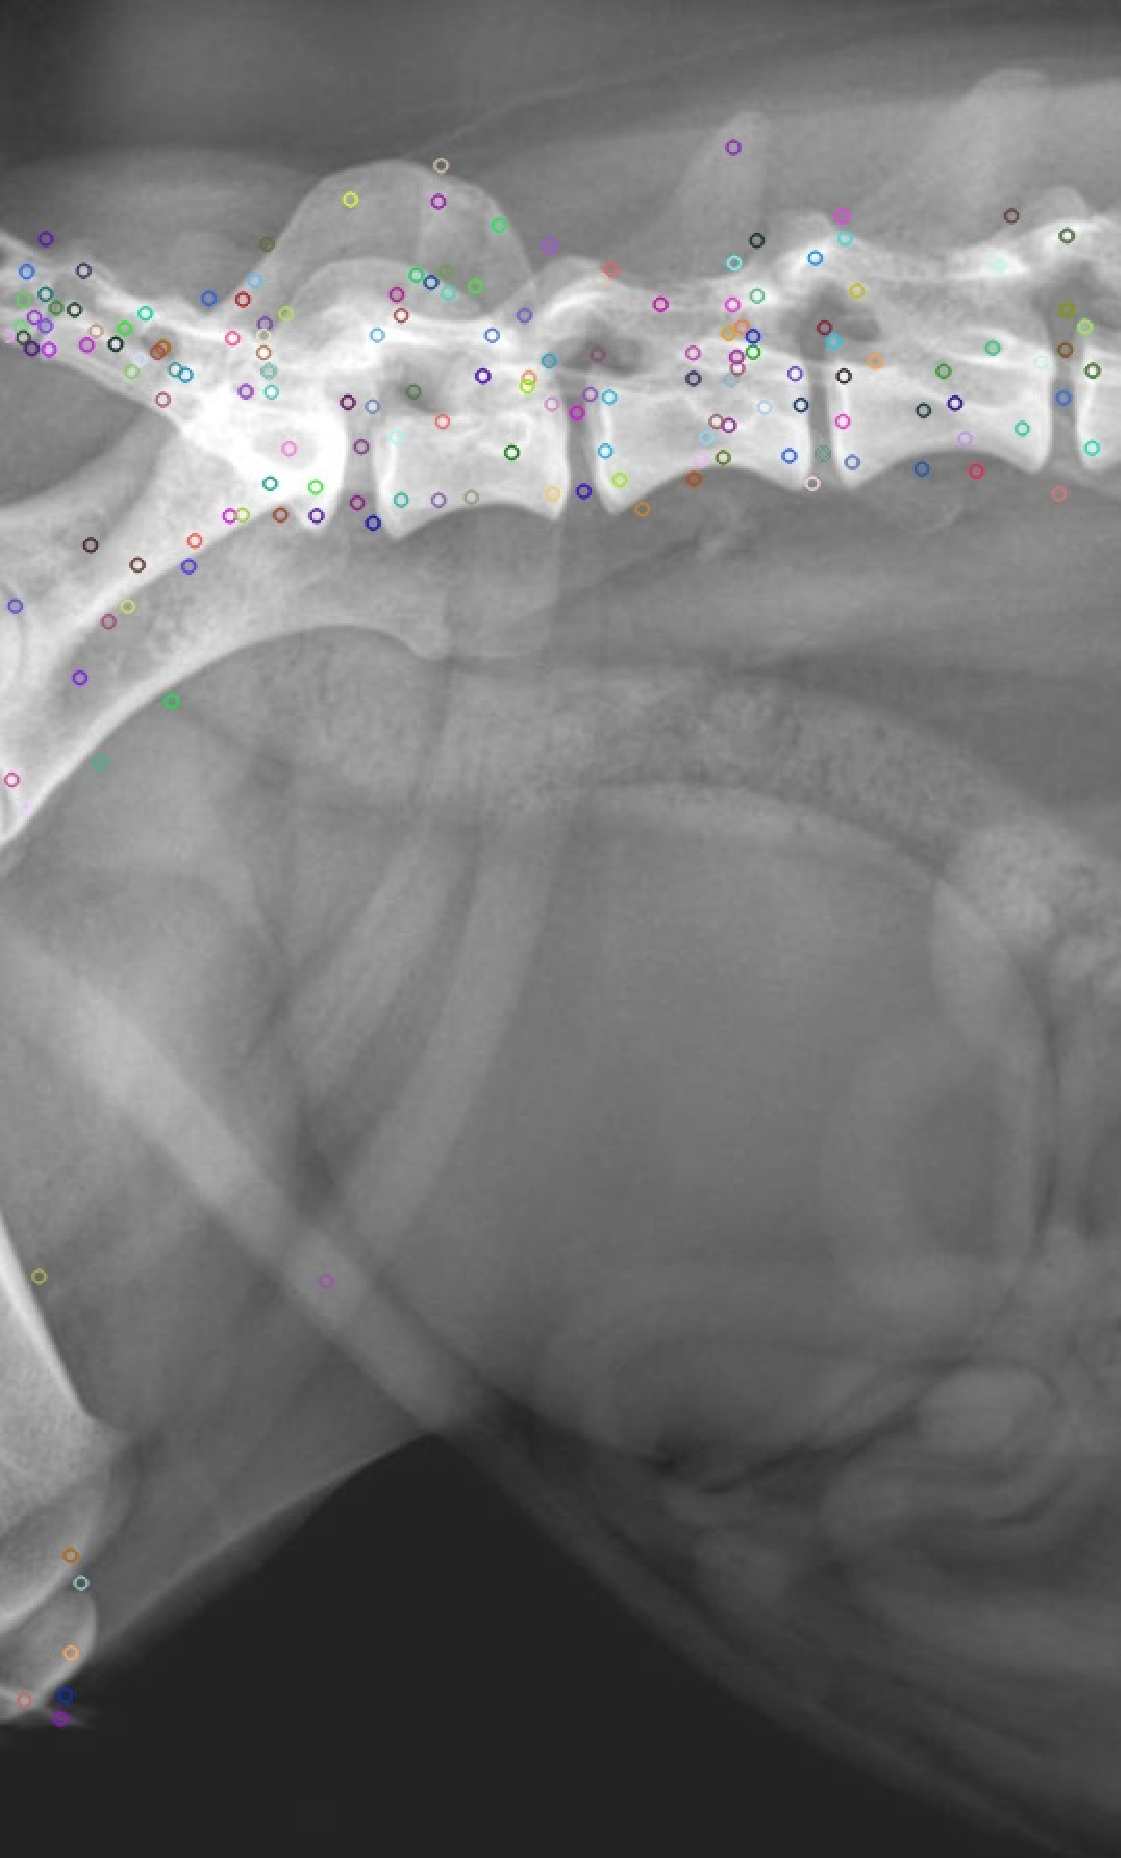
\includegraphics[scale=0.15]{3.backmatter/figures/sift/l_br_rot}}
	%\subfloat[]{\label{fig:intensity-scaling} 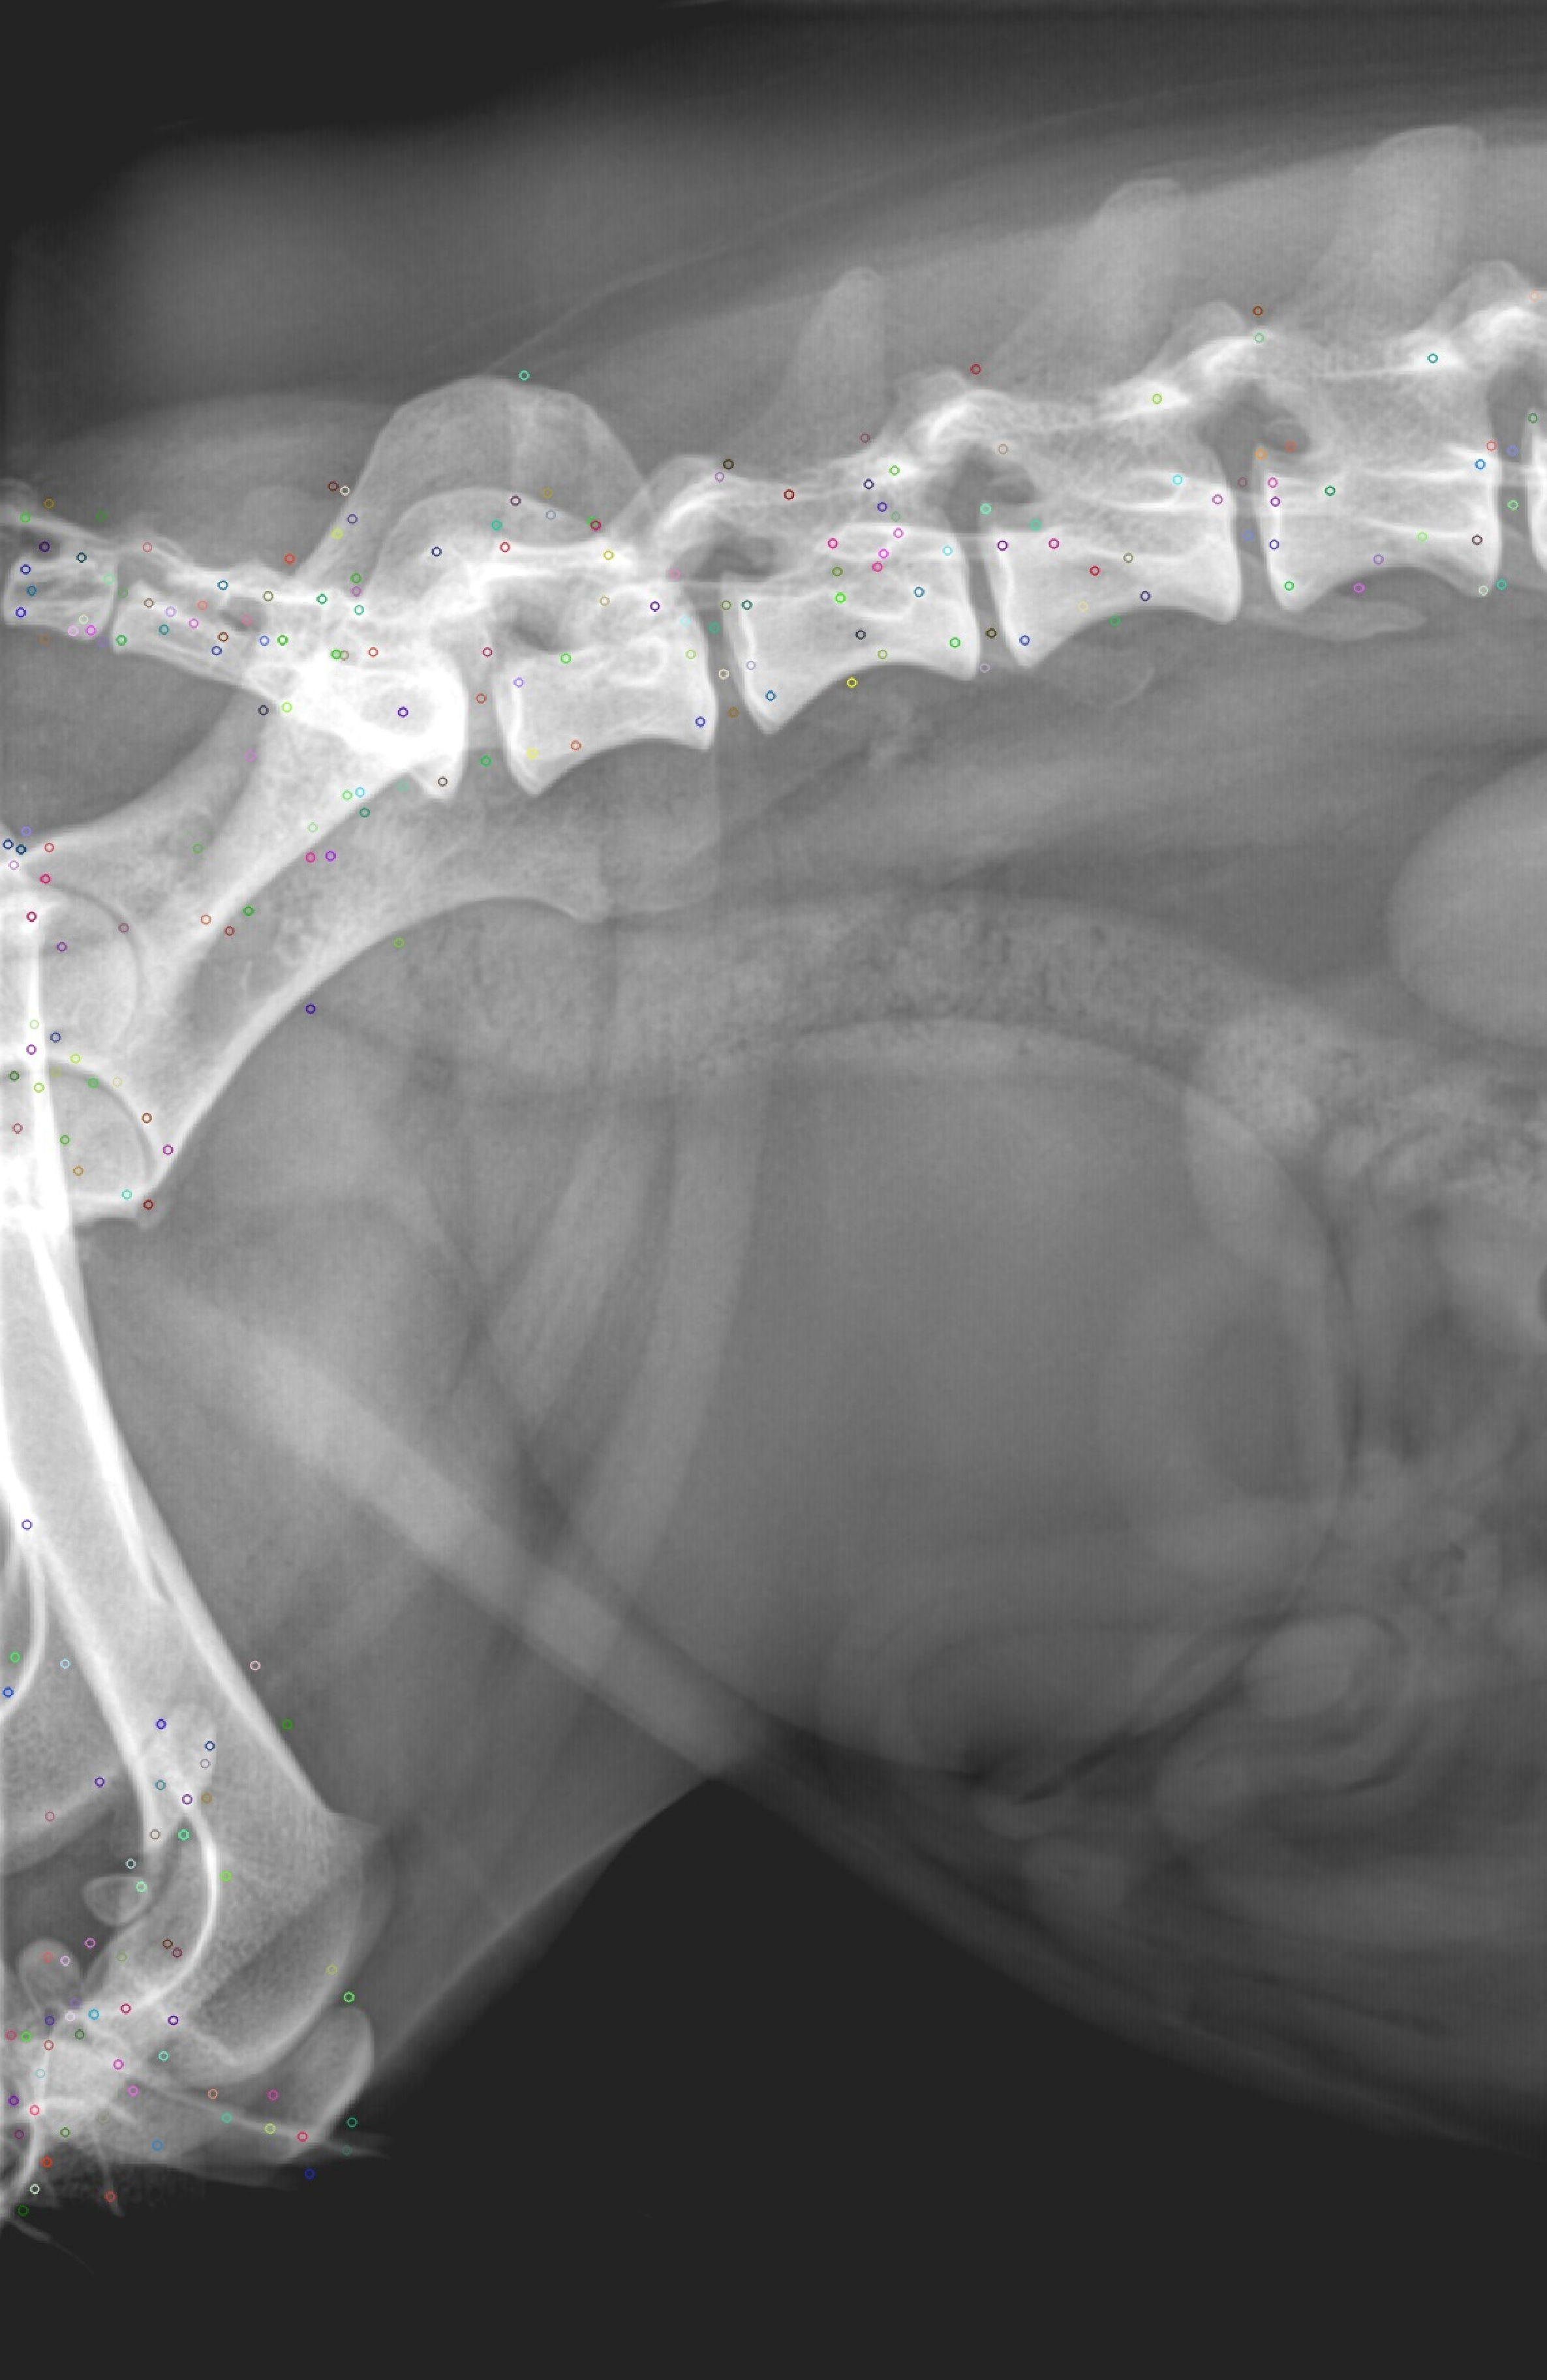
\includegraphics[scale=0.10]{3.backmatter/figures/sift/l_large_br}} 
	%\subfloat[]{\label{fig:intensity-rotation-scaling} 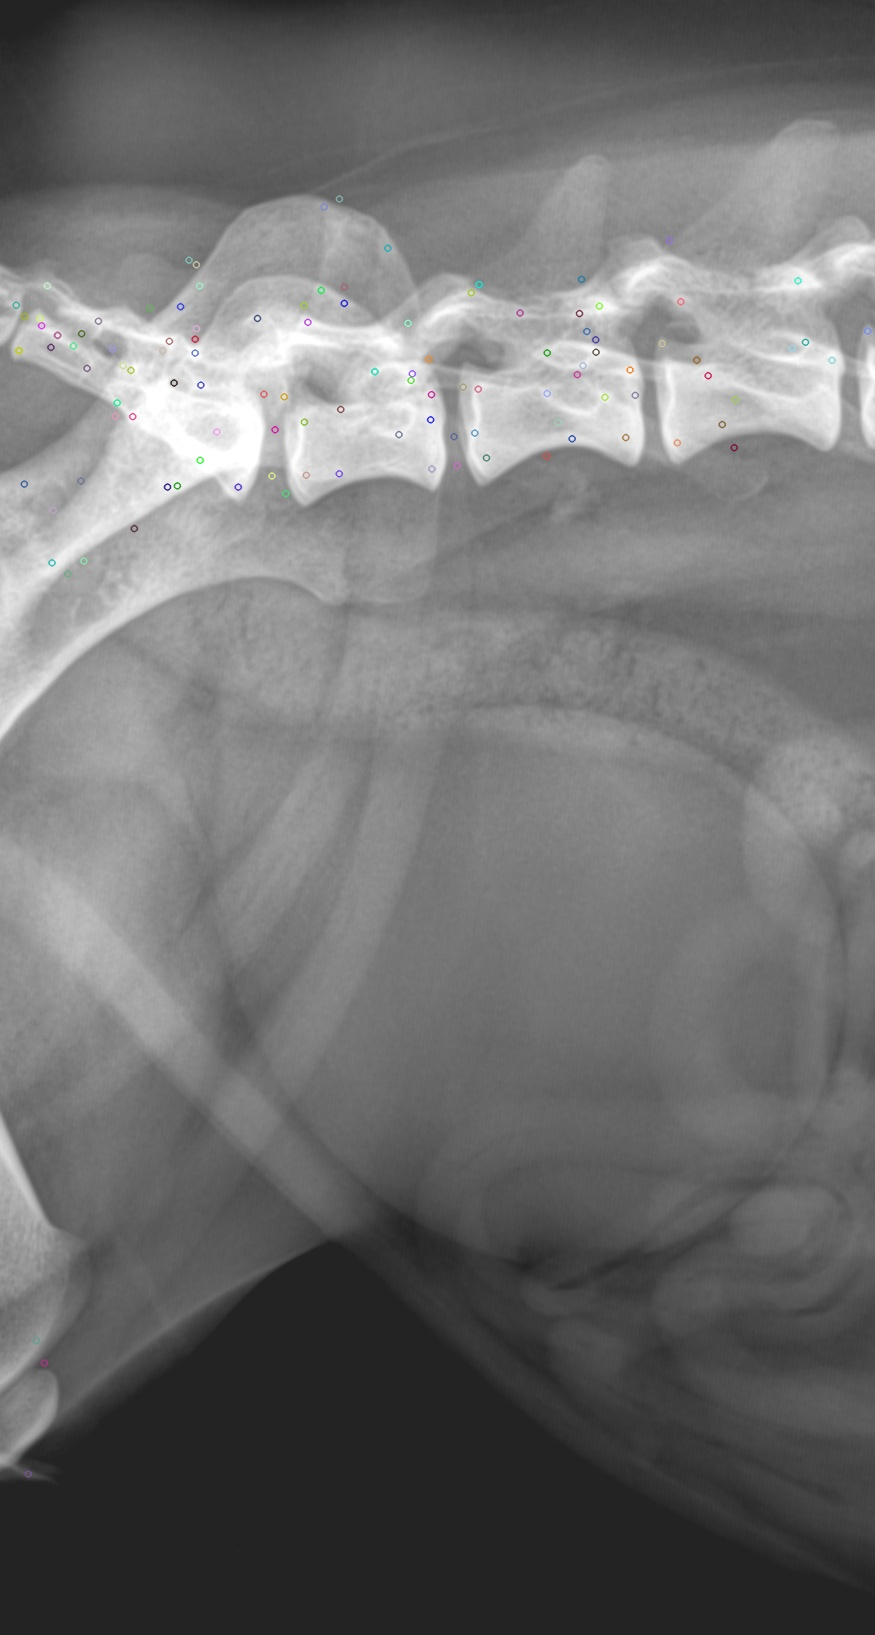
\includegraphics[scale=0.10]{3.backmatter/figures/sift/l_large_br_rot}} 
	%\subfloat[]{\label{fig:noisy} 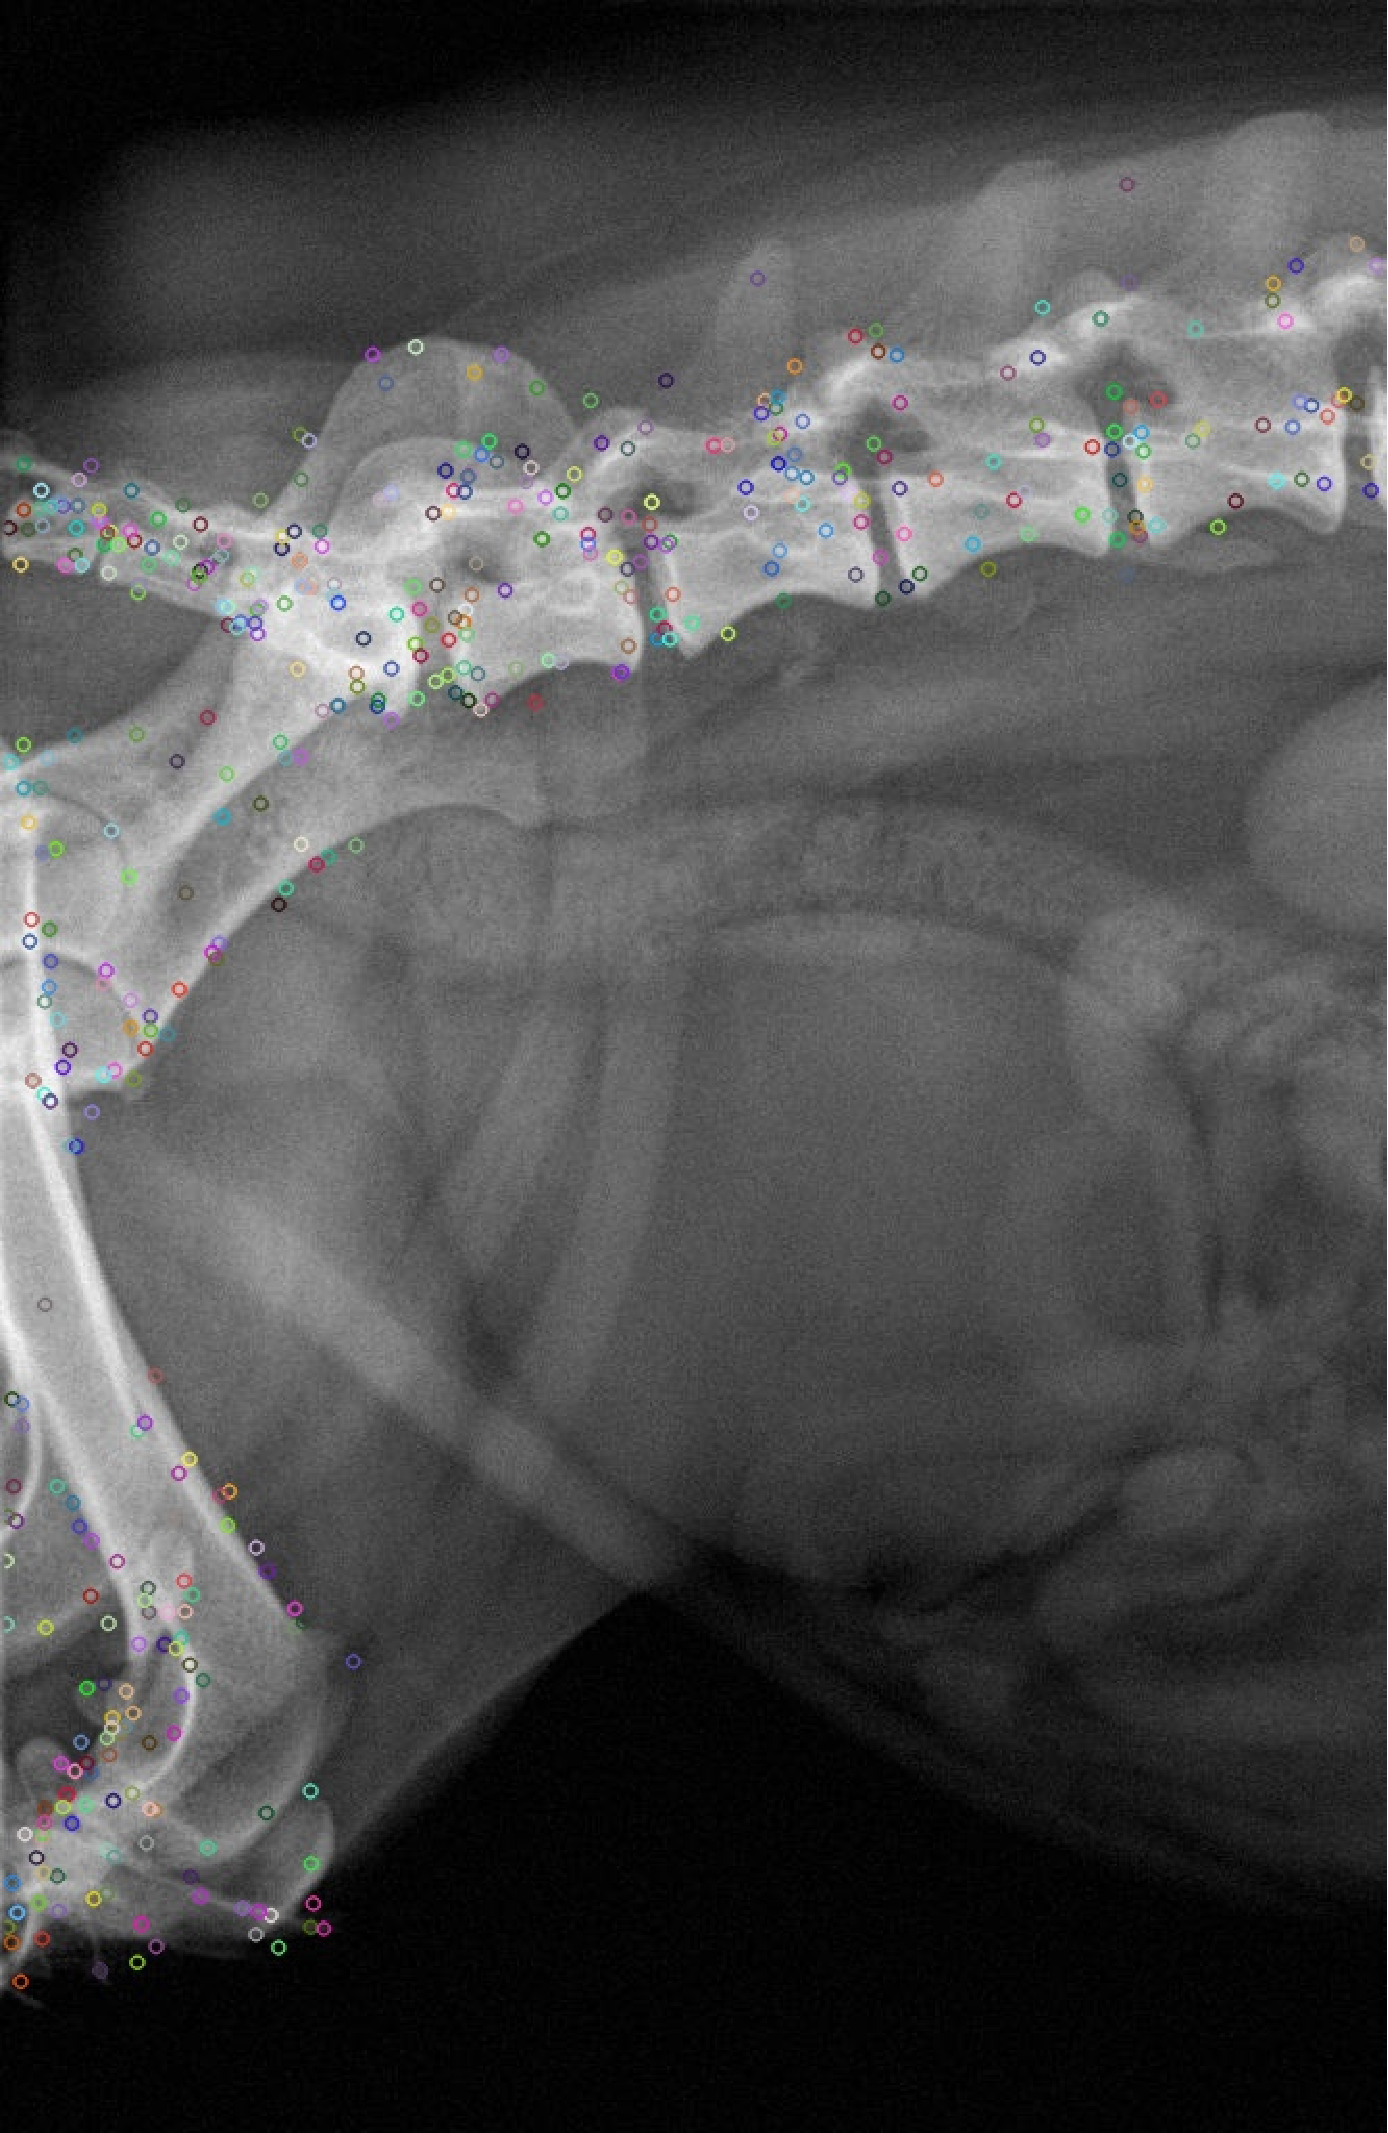
\includegraphics[scale=0.15]{3.backmatter/figures/sift/l_noise}}  
\end{center}
\caption[Result of SIFT]{Result of SIFT feature extractor. \subref{fig:original-image}Original Image, \subref{fig:intensity-change}Image with increased intensity, \subref{fig:rotation}Rotated image \subref{fig:scaled}Scaled image}% \subref{fig:intensity-rotation}Increase intensity \& rotation \subref{fig:intensity-scaling}Increased intensity \& scaling \subref{fig:intensity-rotation-scaling}Increased intensity, rotation \& scaling \subref{fig:noisy}Noisy image}
\end{figure}


\subsection{SURF}
\begin{figure}[H]%
\begin{center}
	\subfloat[]{\label{fig:original-image}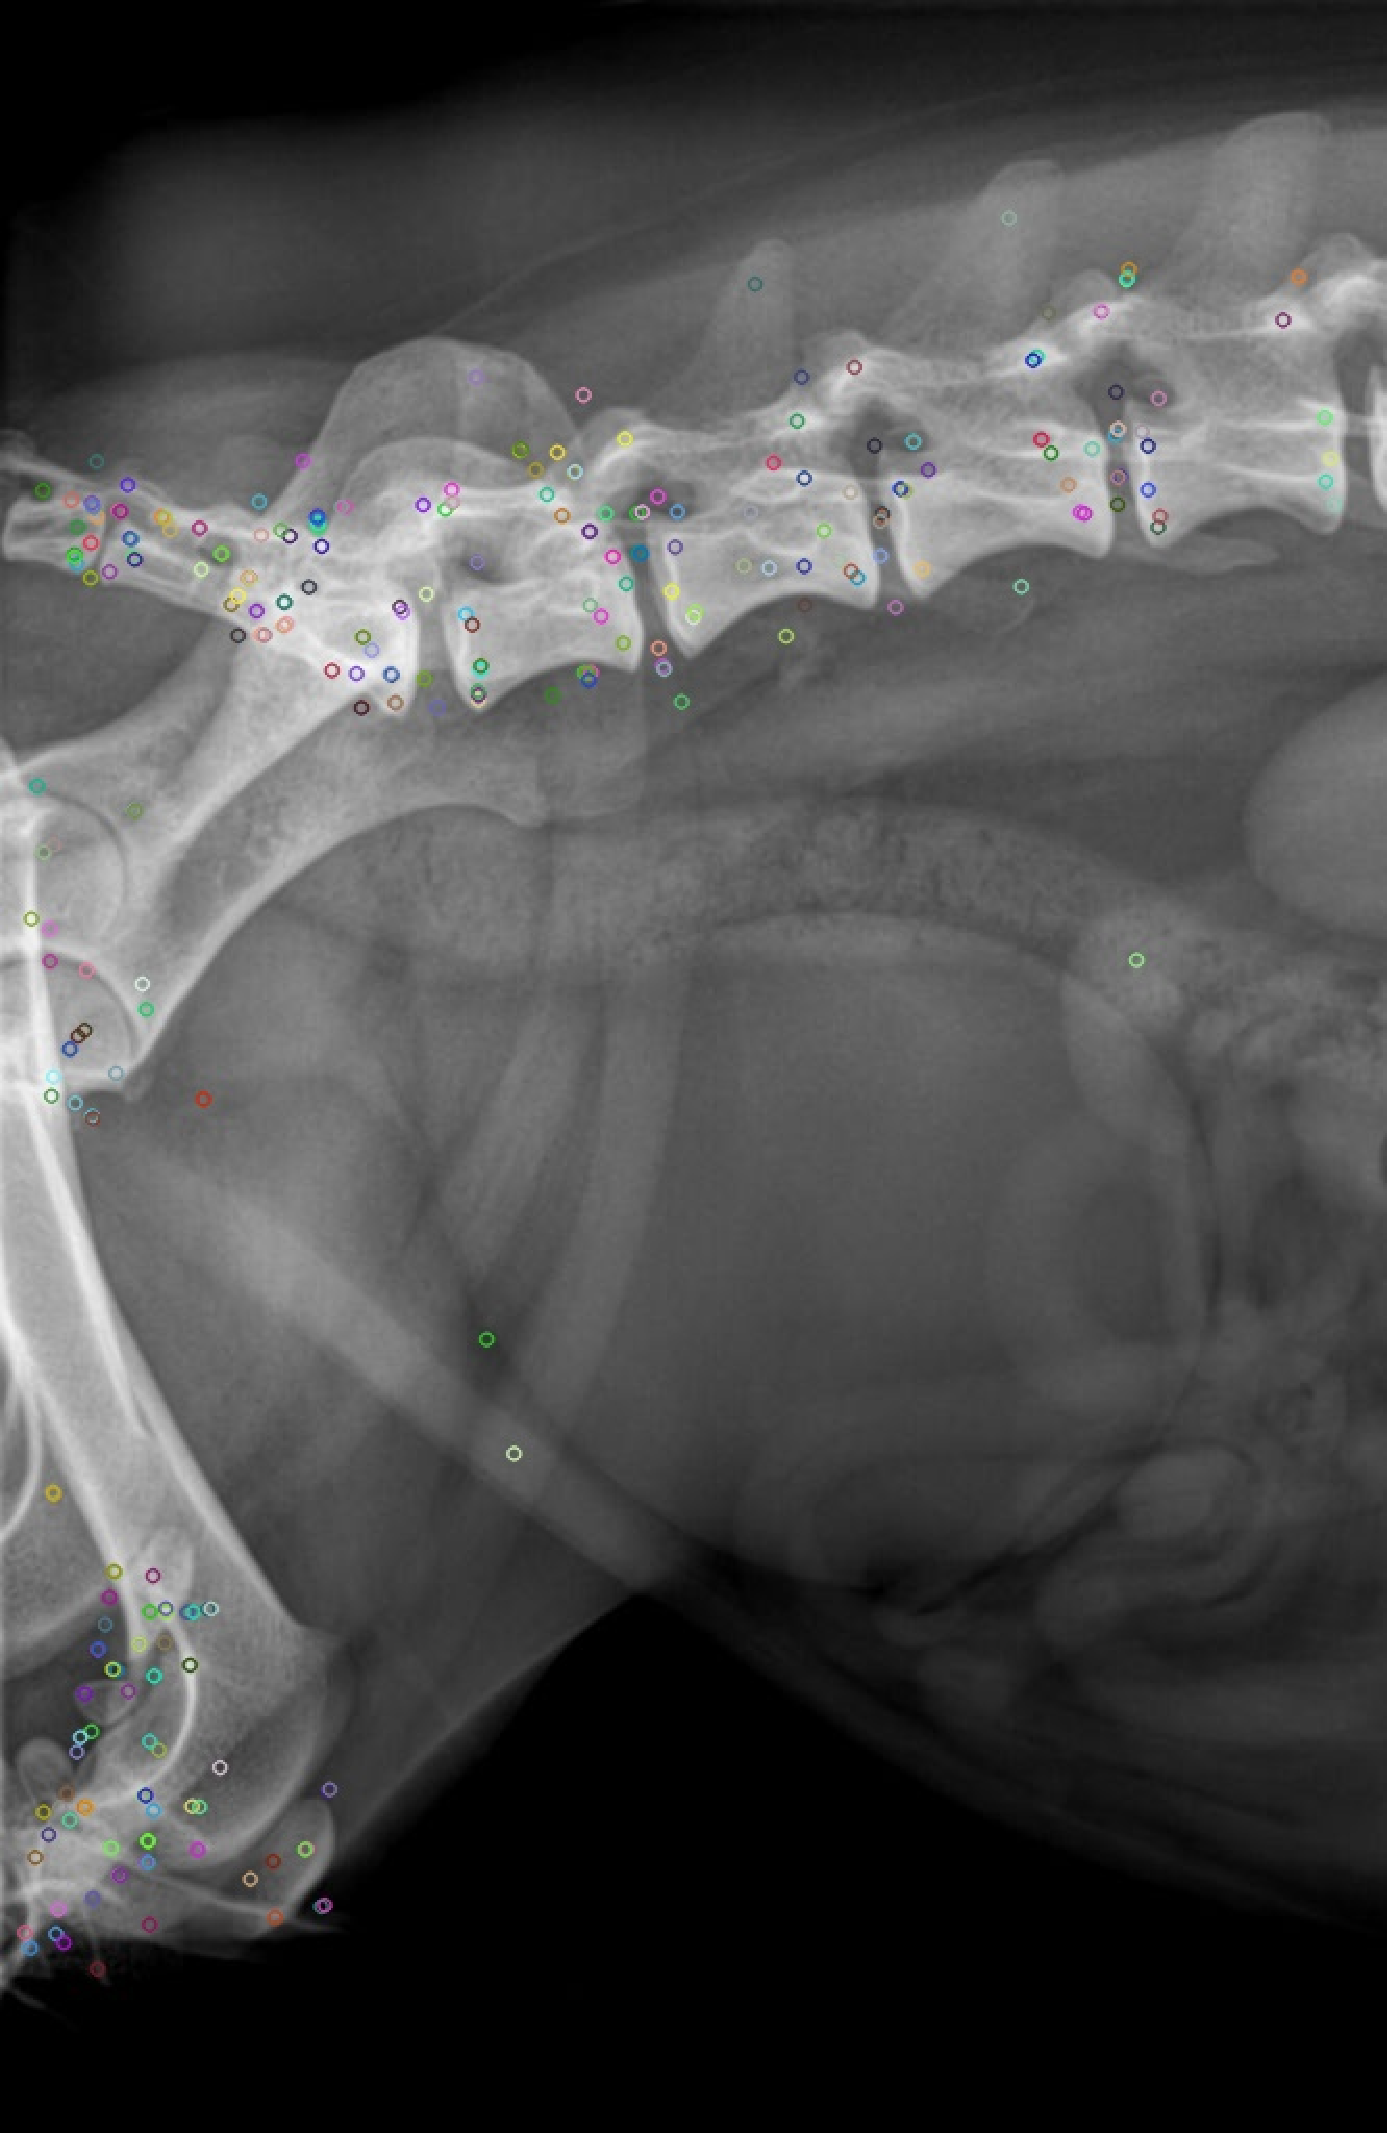
\includegraphics[scale=0.20]{3.backmatter/figures/surf/l}} 
	\subfloat[]{\label{fig:intensity-change} 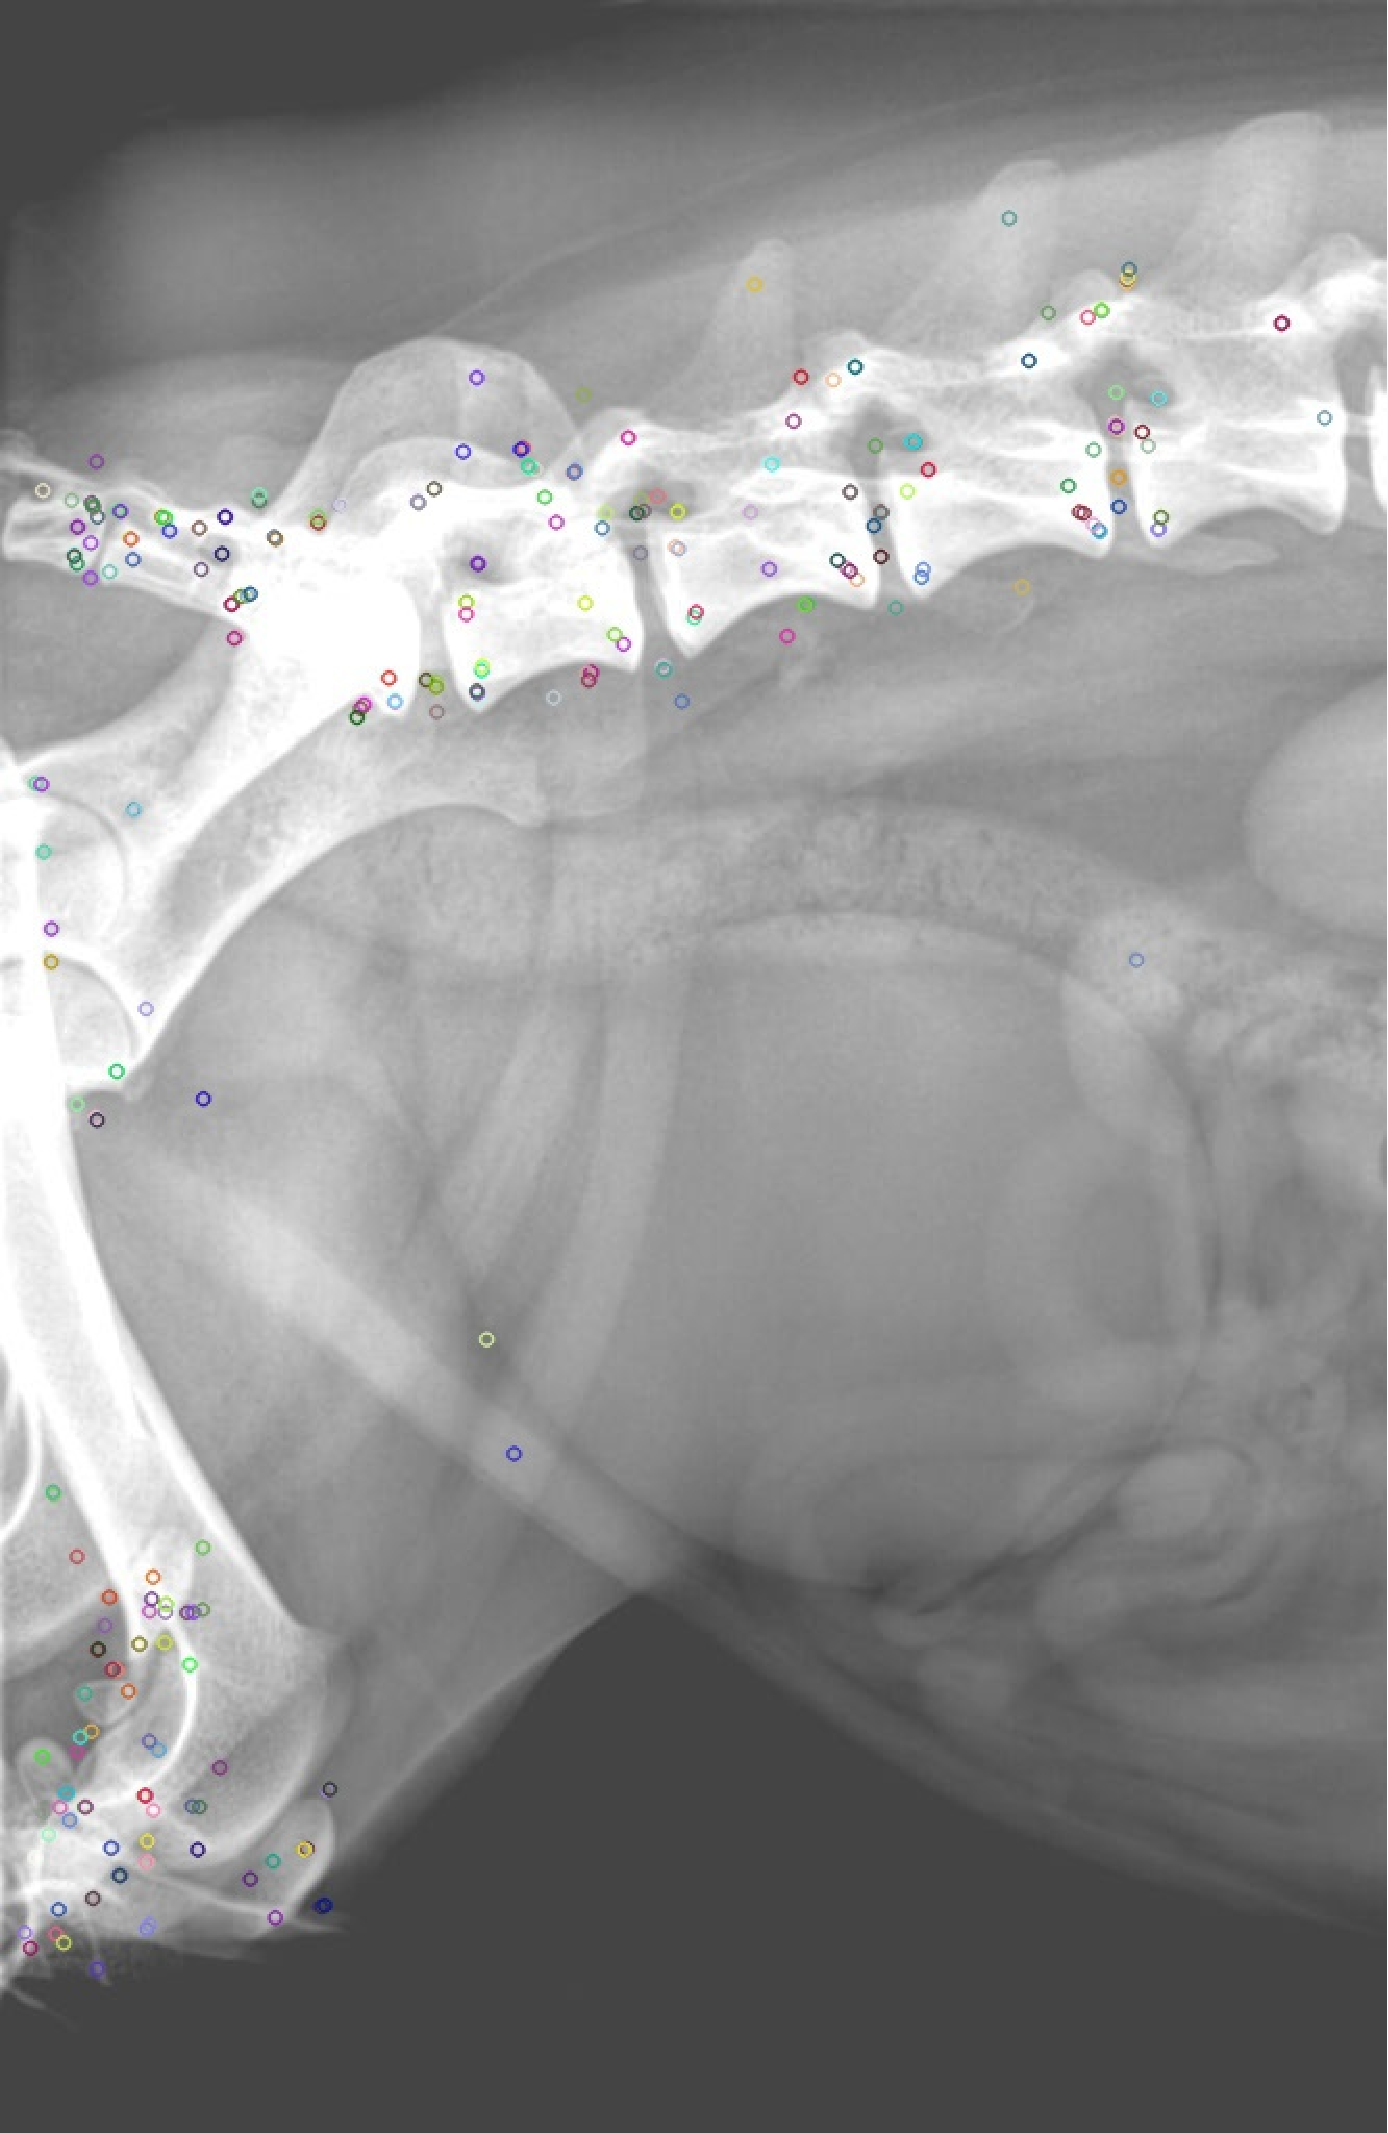
\includegraphics[scale=0.20]{3.backmatter/figures/surf/l_br}}  \quad
	\subfloat[]{\label{fig:rotation} 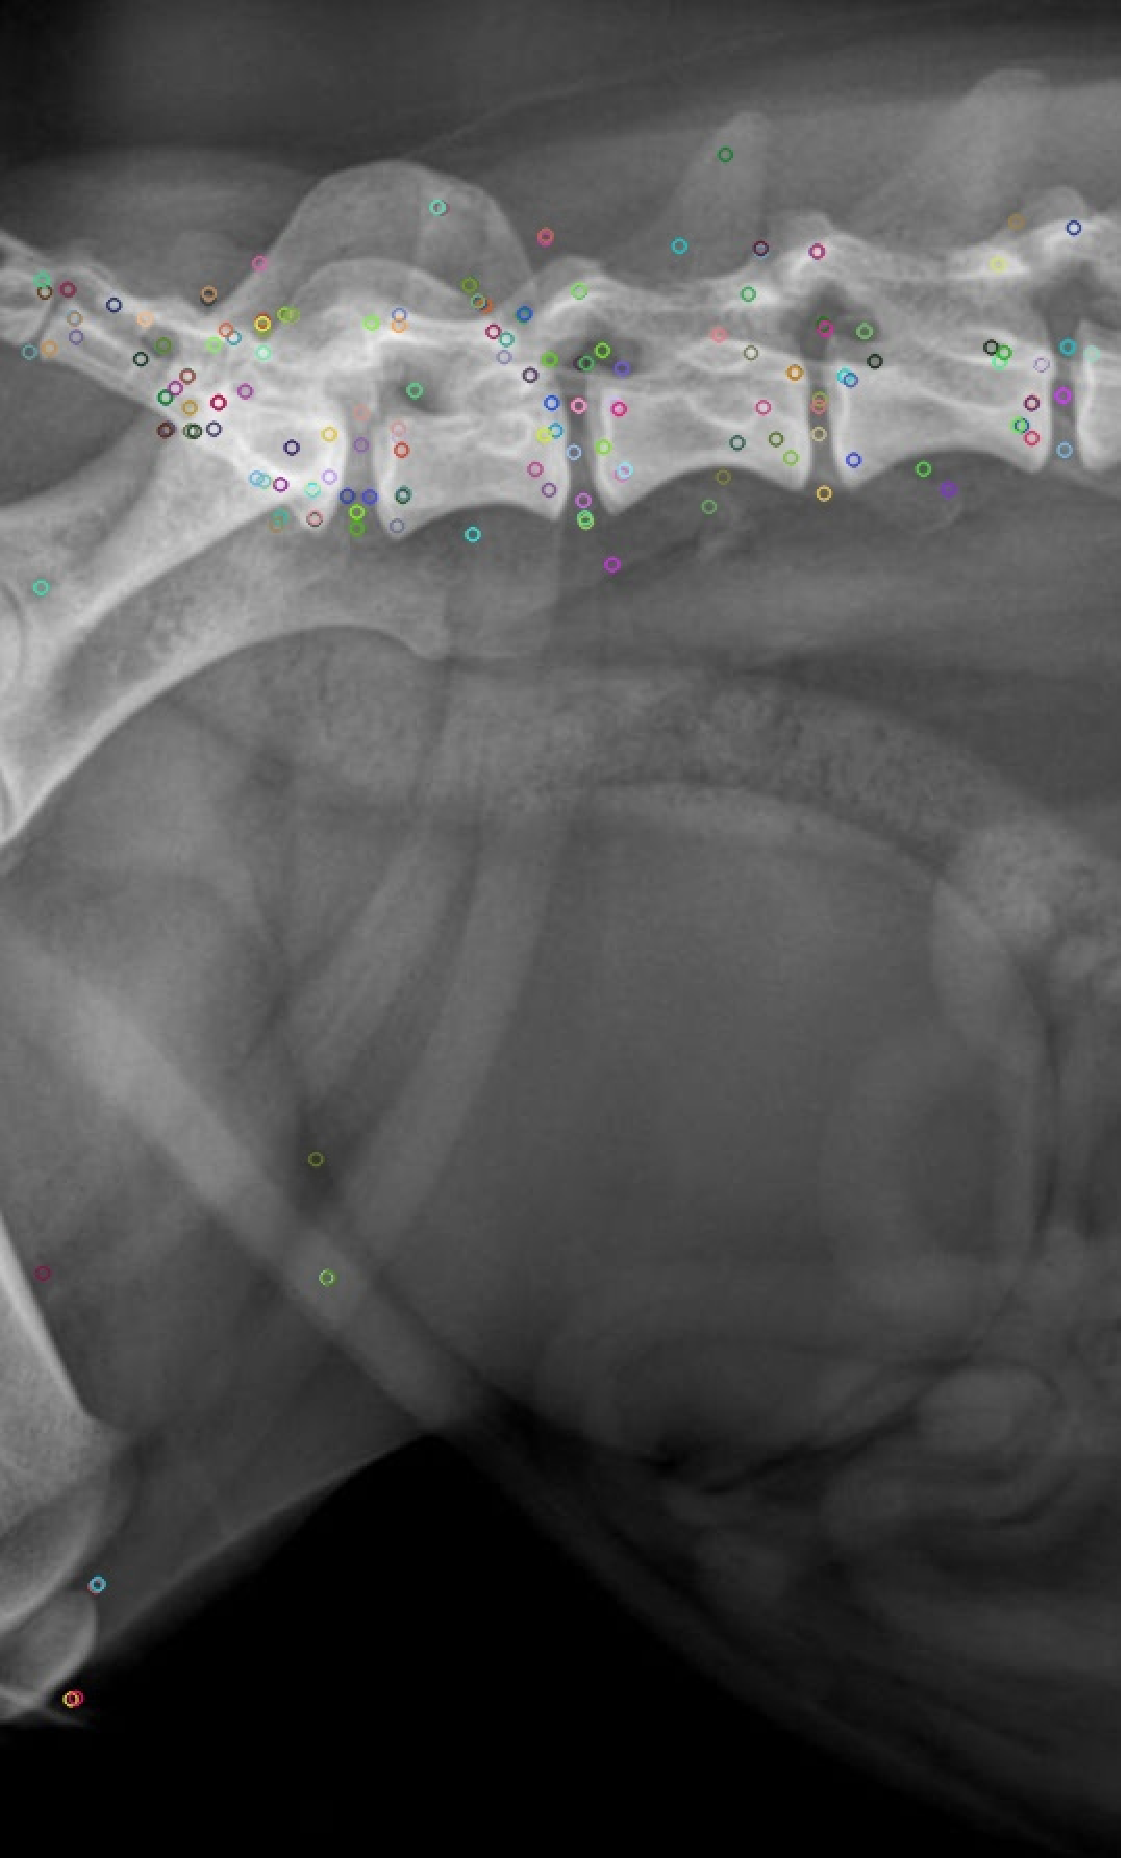
\includegraphics[scale=0.25]{3.backmatter/figures/surf/l_rot_8}}	
	\subfloat[]{\label{fig:scaled} 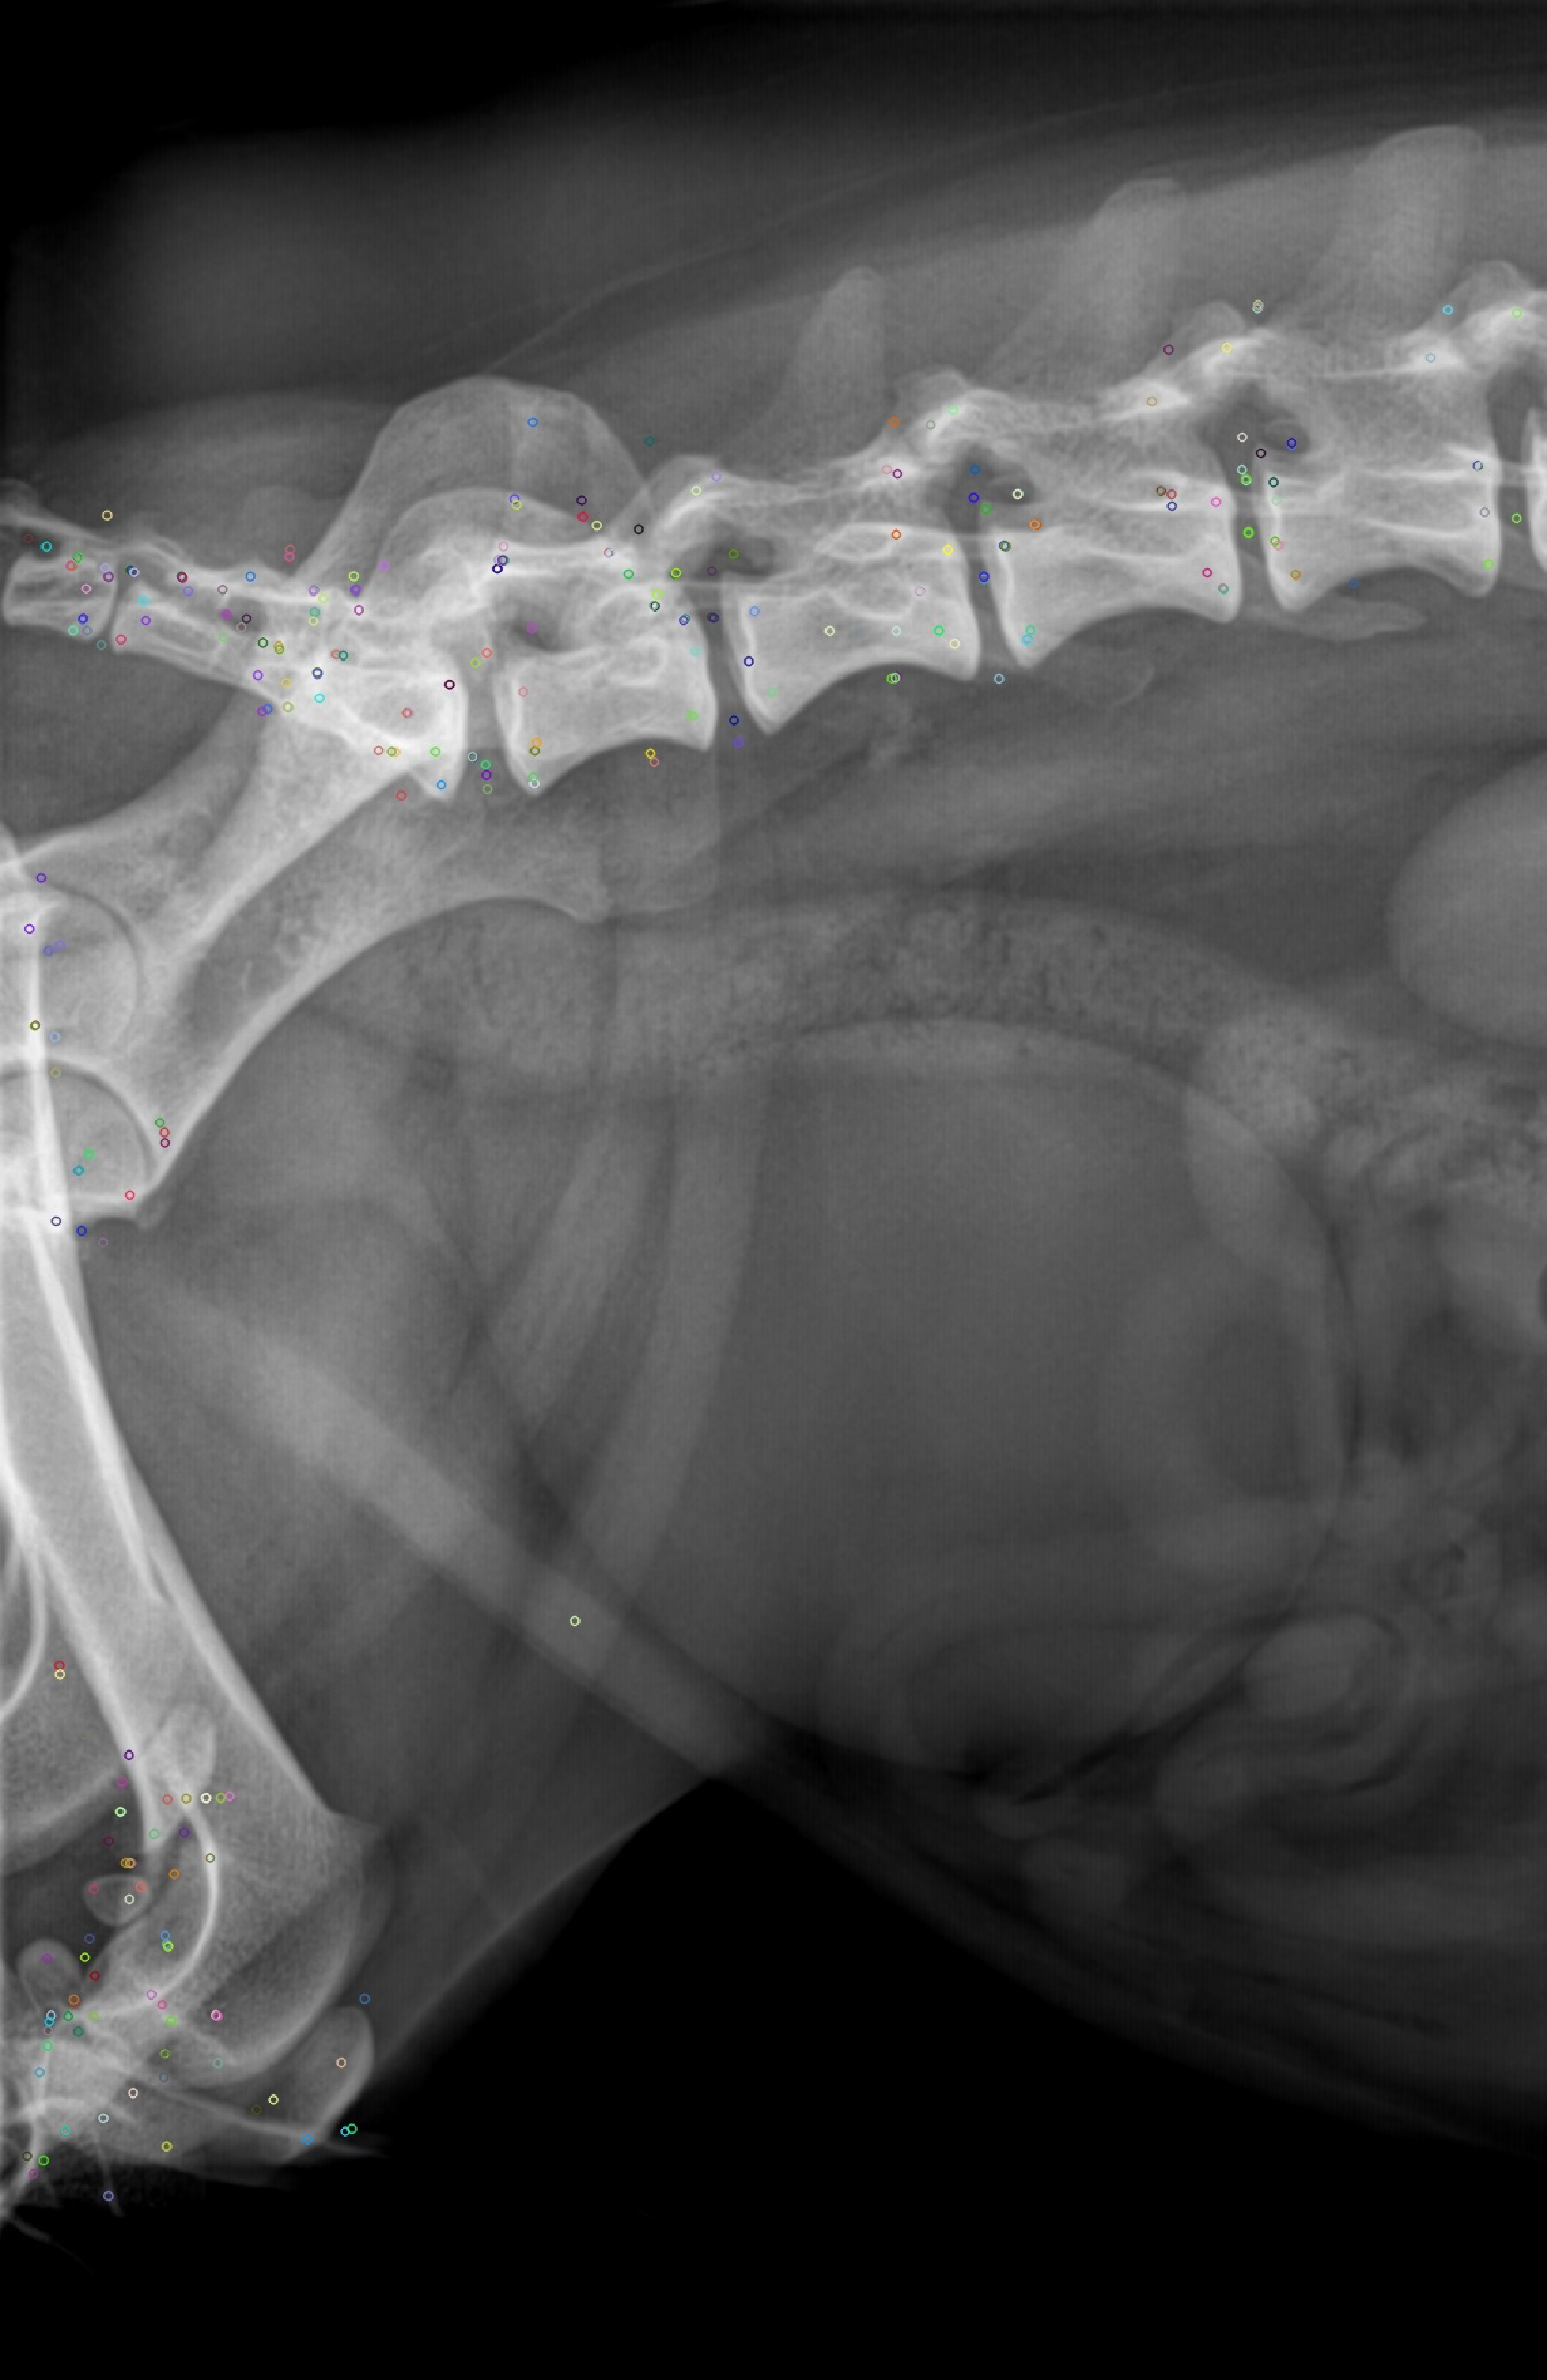
\includegraphics[scale=0.15]{3.backmatter/figures/surf/l_large}} 	
	%\subfloat[]{\label{fig:intensity-rotation} 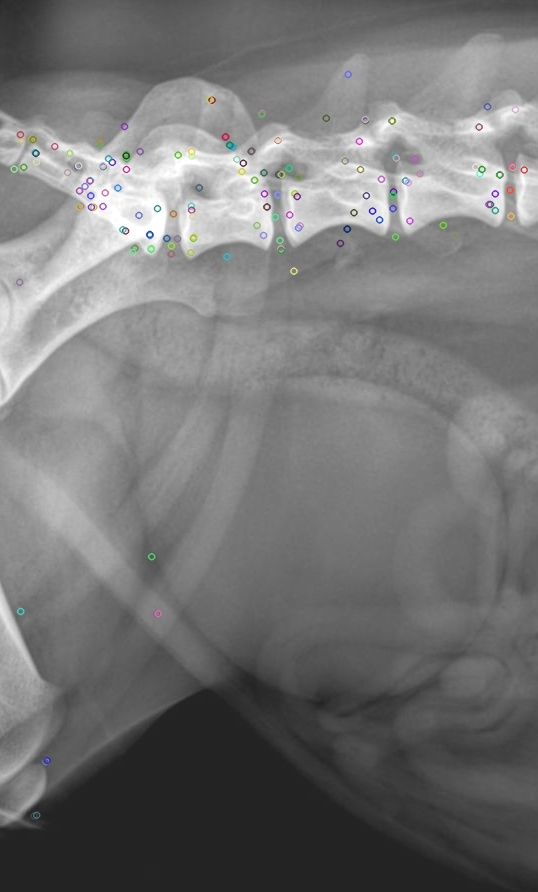
\includegraphics[scale=0.15]{3.backmatter/figures/surf/l_br_rot}}
	%\subfloat[]{\label{fig:intensity-scaling} 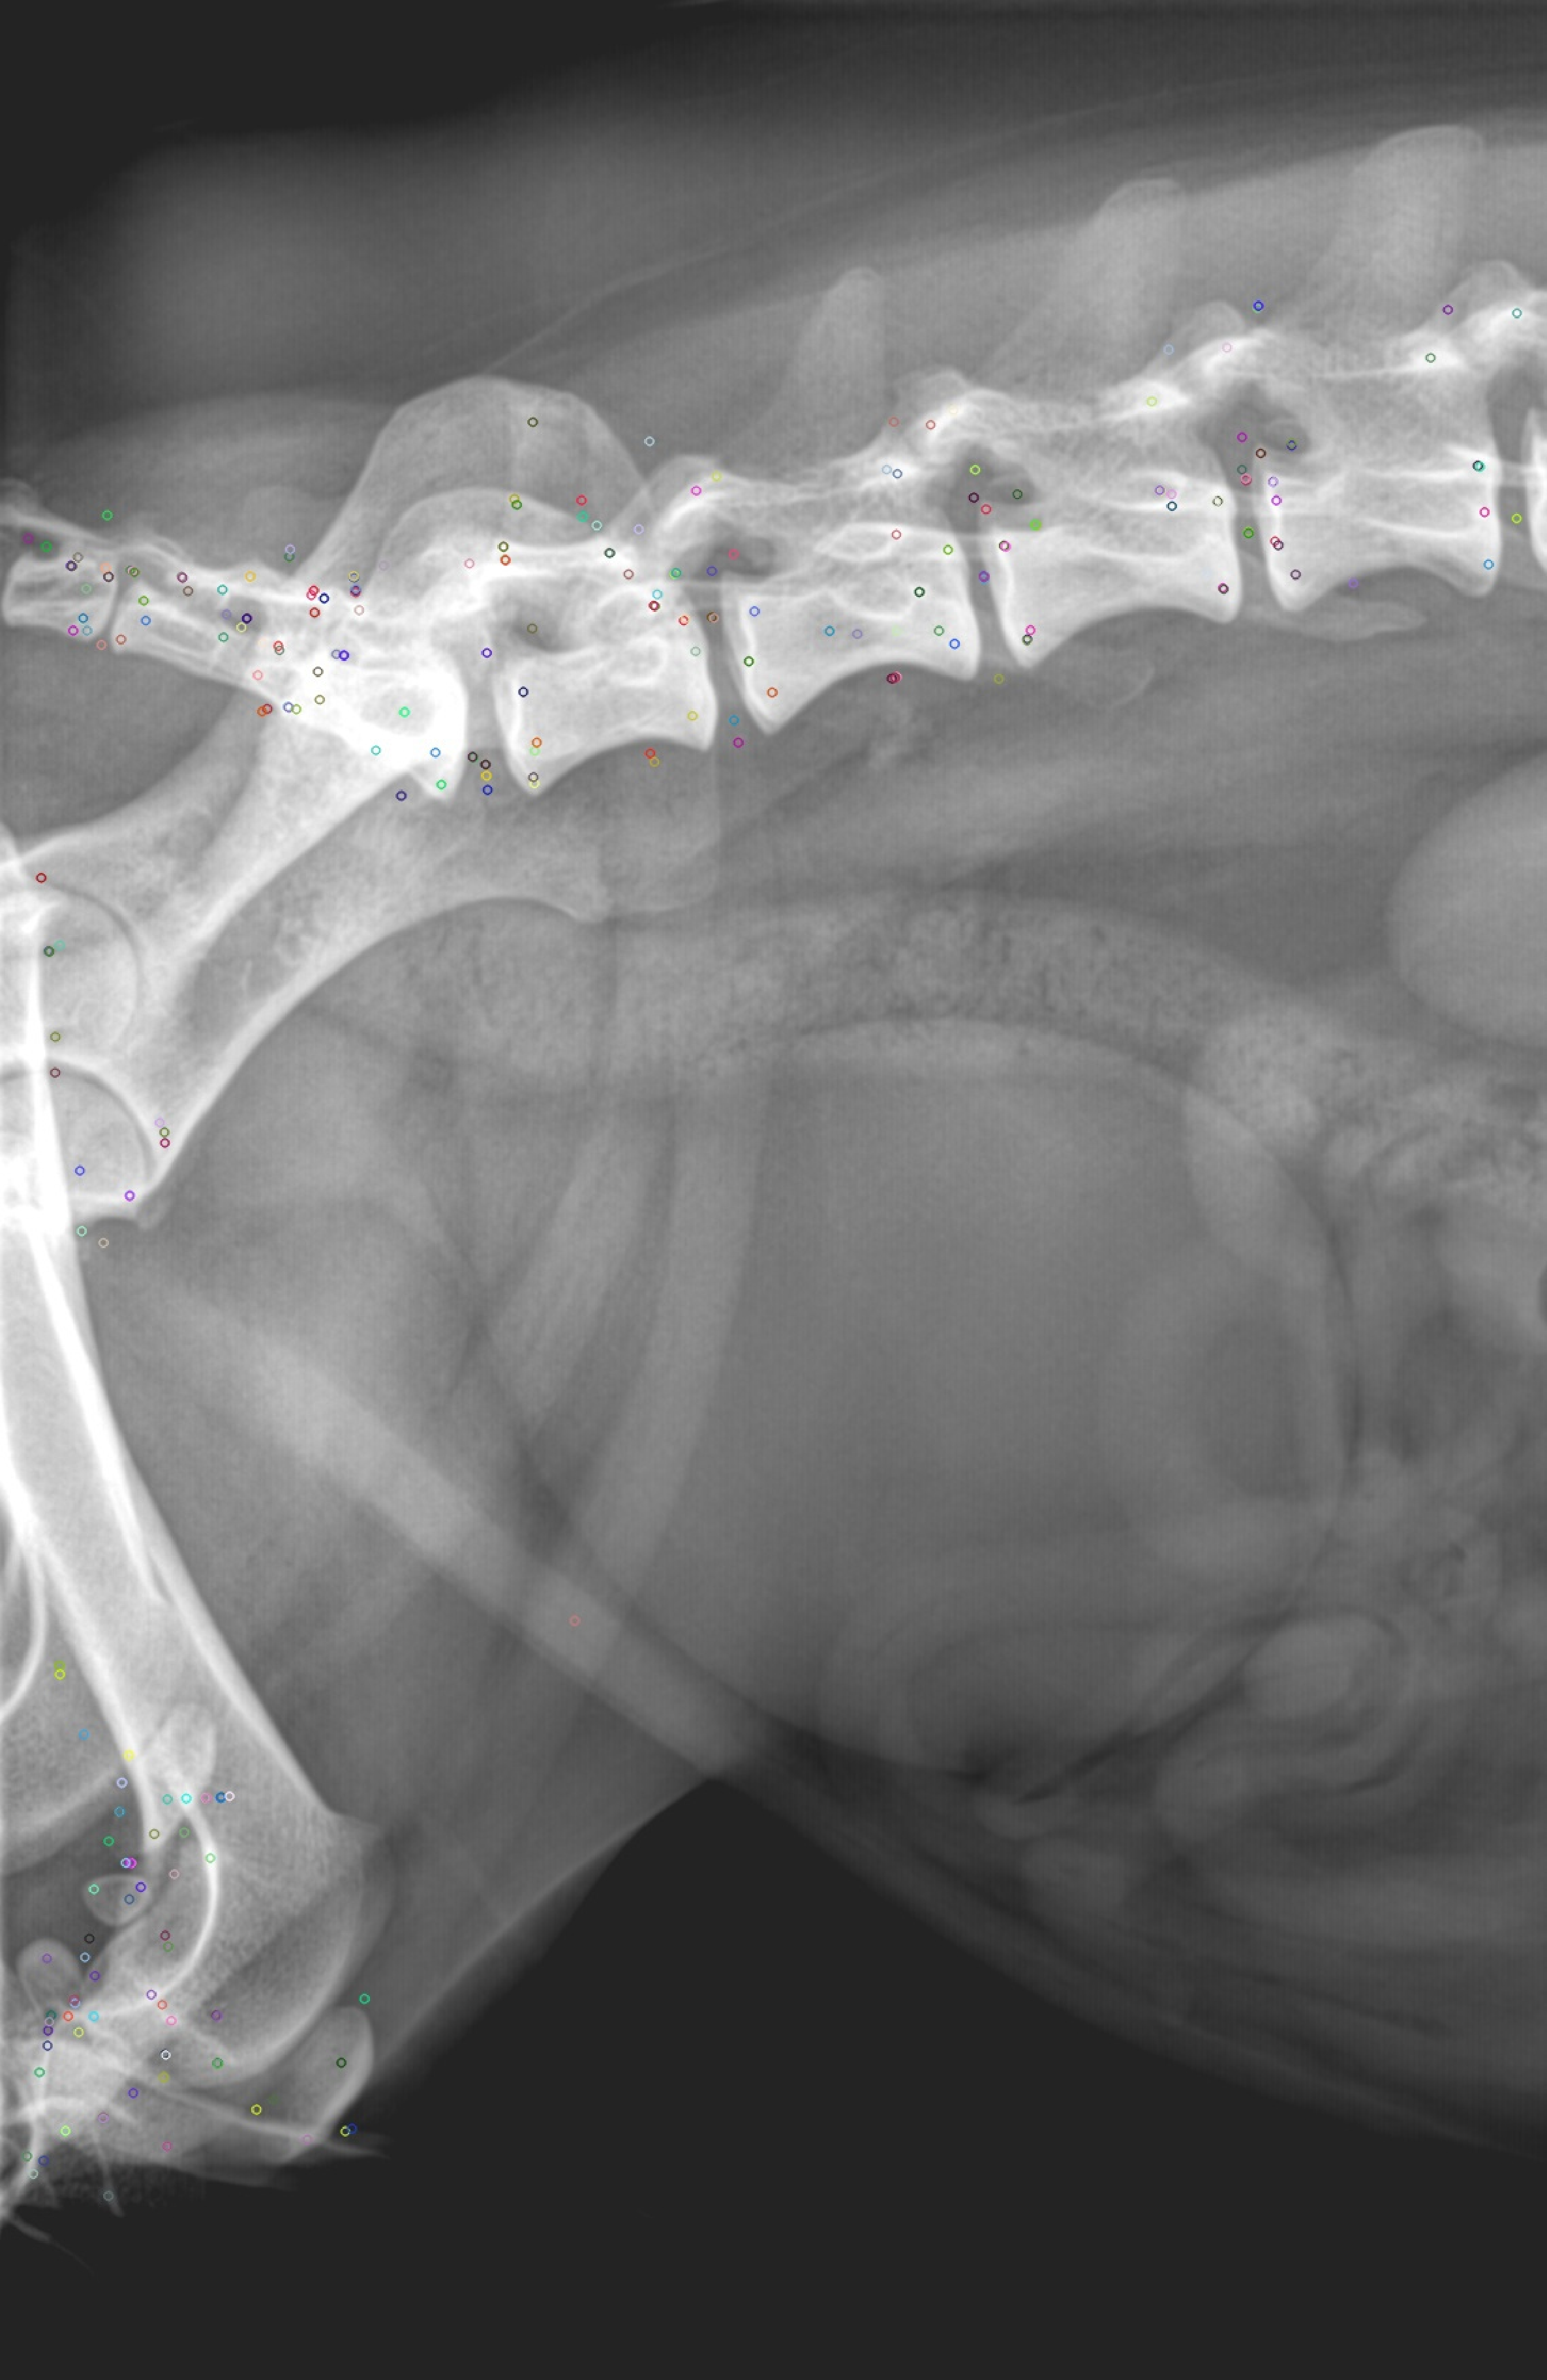
\includegraphics[scale=0.10]{3.backmatter/figures/surf/l_large_br}} 
	%\subfloat[]{\label{fig:intensity-rotation-scaling} 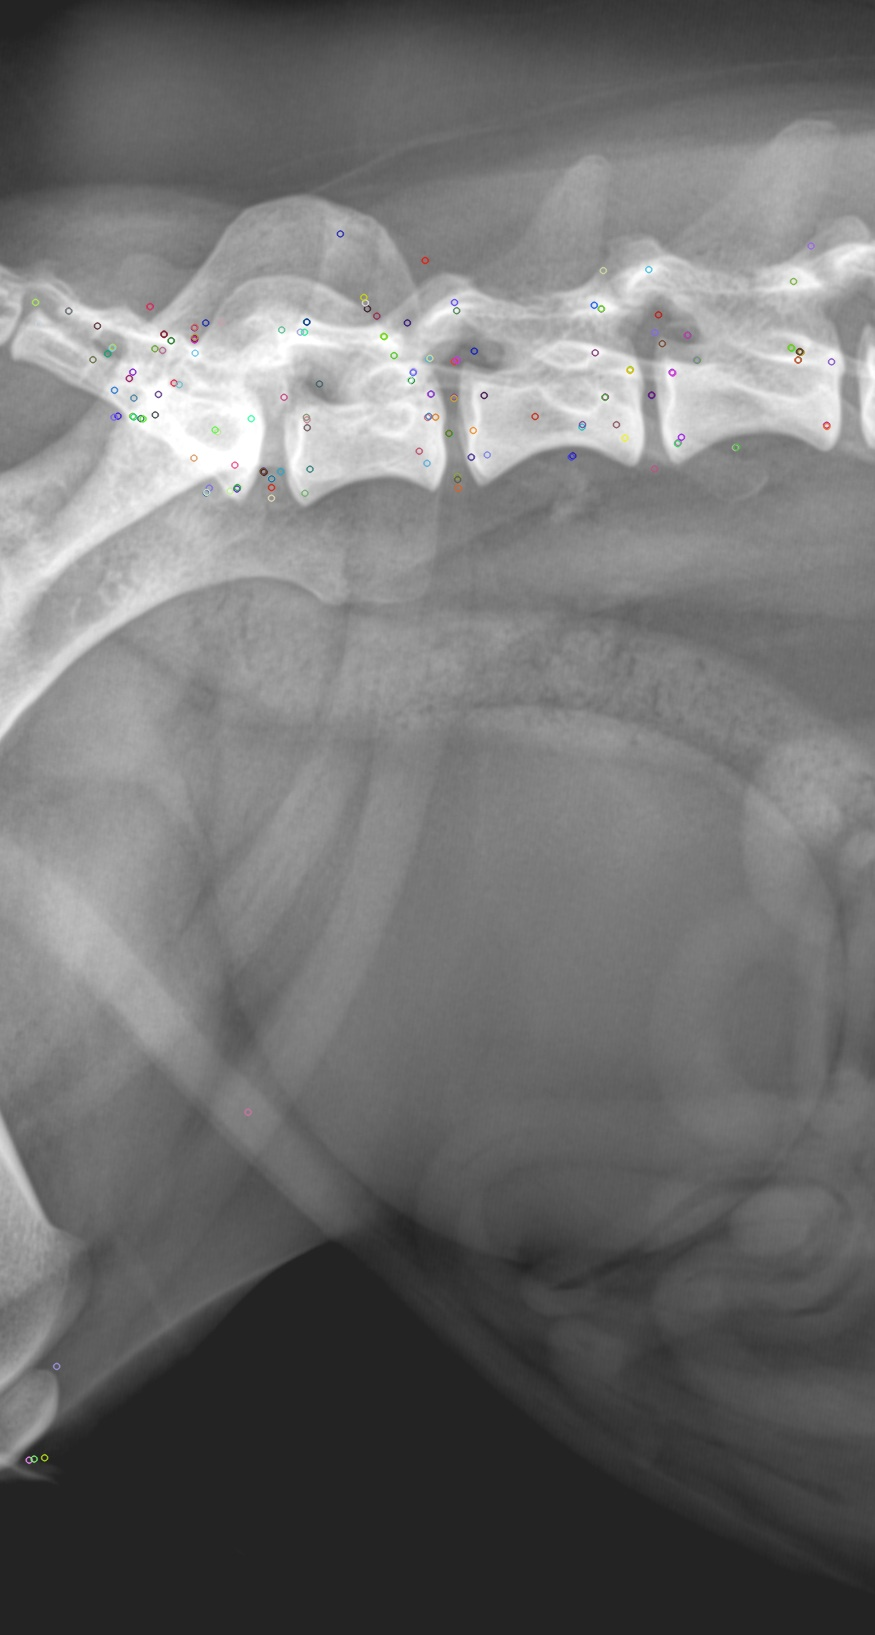
\includegraphics[scale=0.10]{3.backmatter/figures/surf/l_large_br_rot}} 
	%\subfloat[]{\label{fig:noisy} 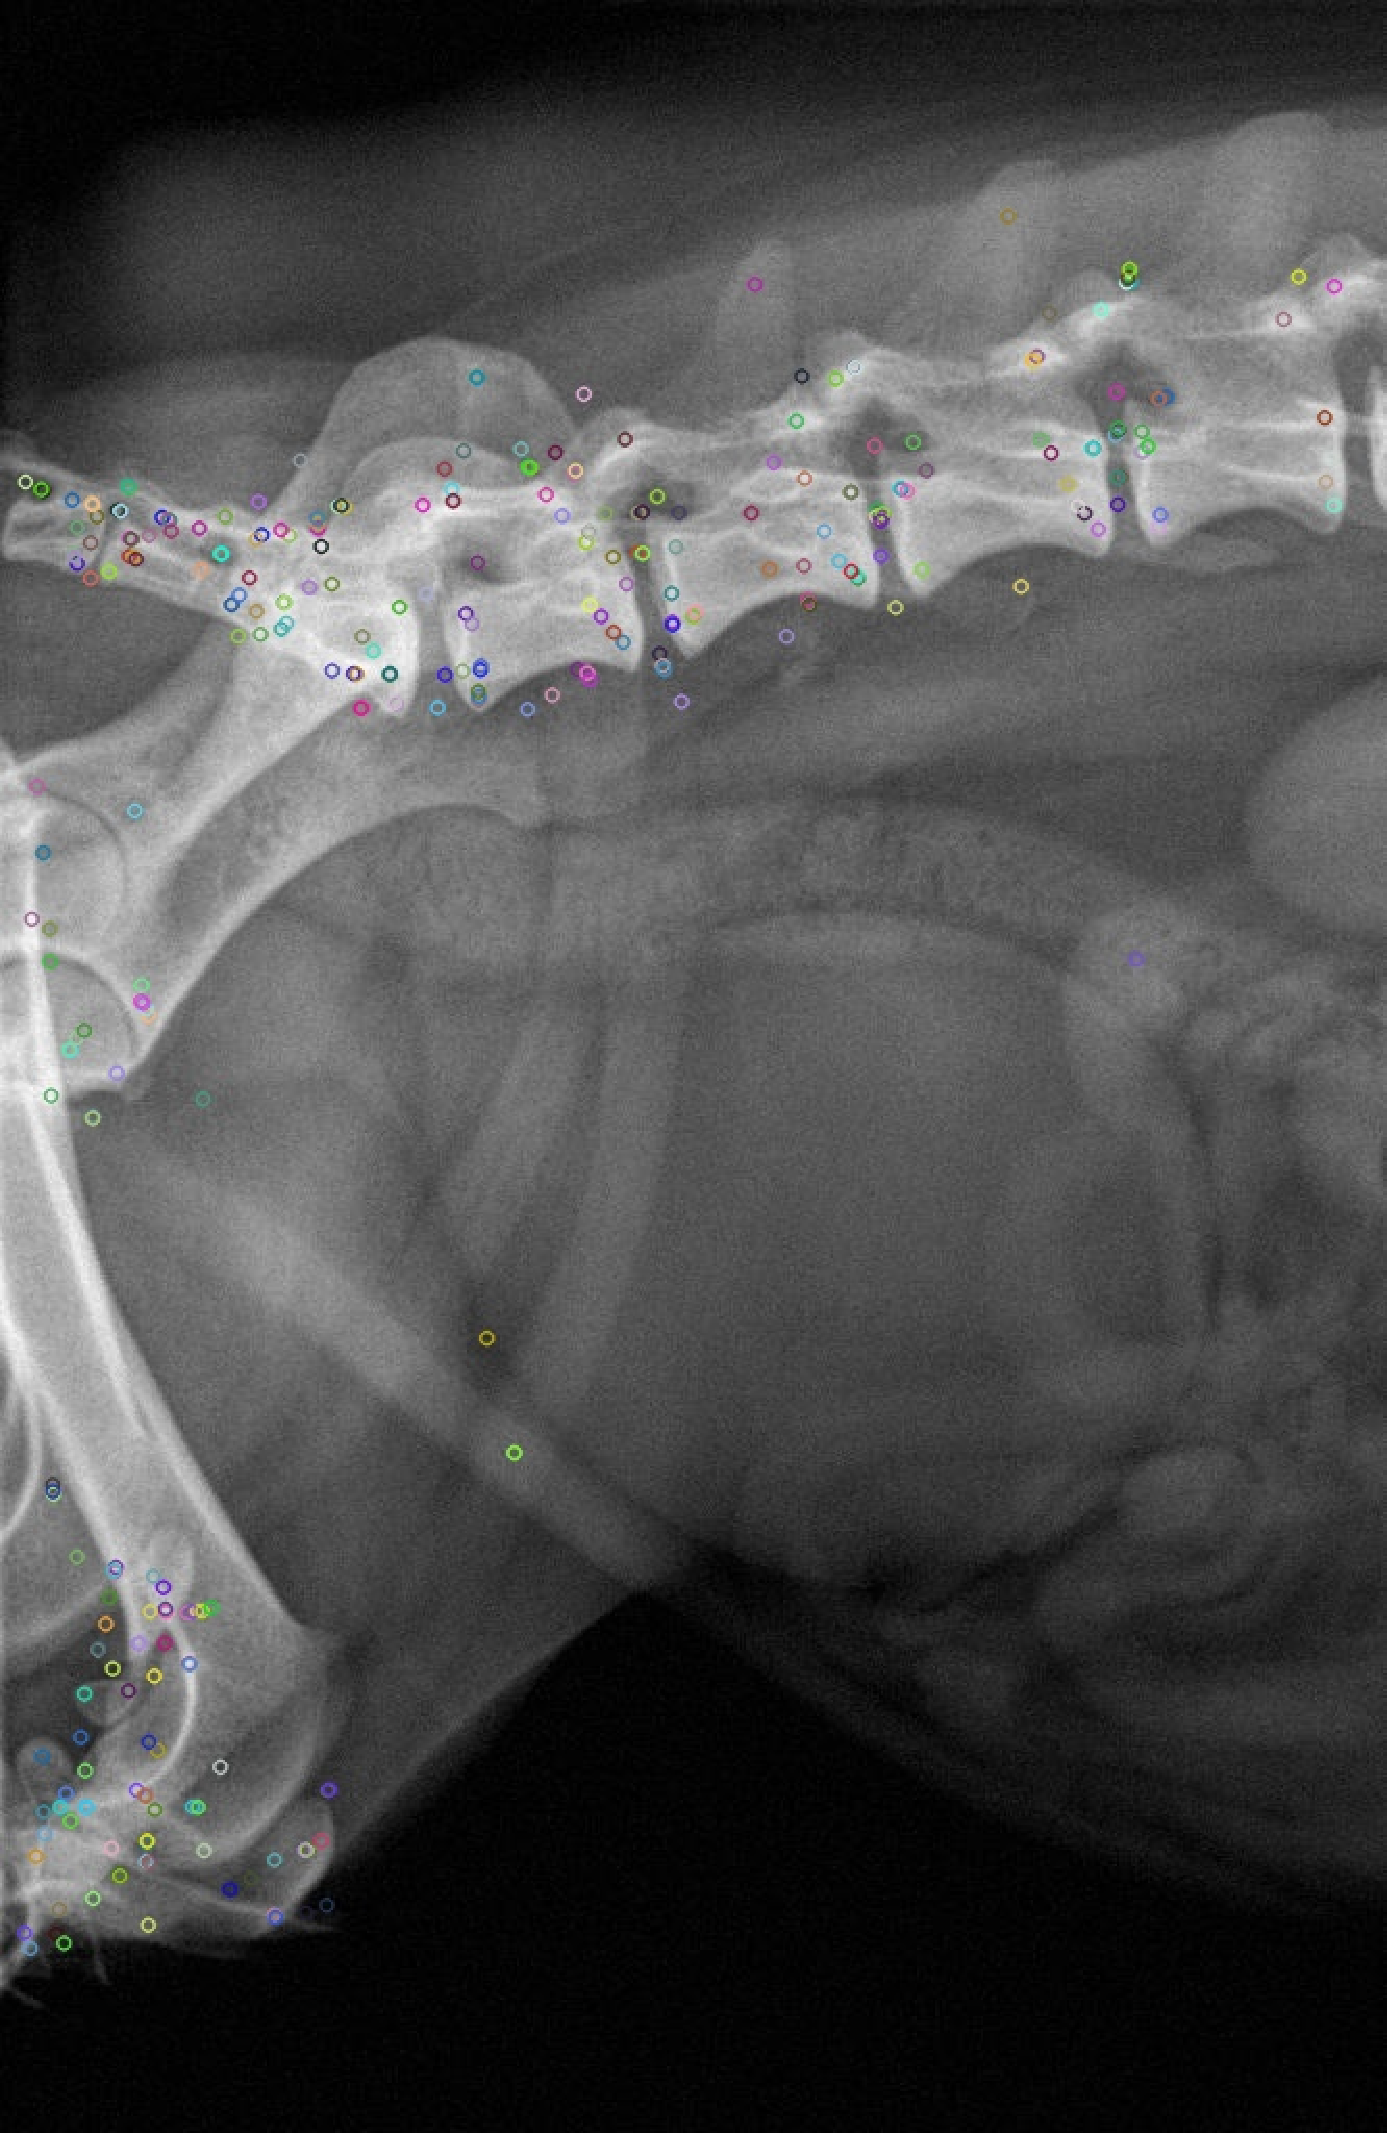
\includegraphics[scale=0.15]{3.backmatter/figures/surf/l_noise}}  
\end{center}
\caption[Result of SURF]{Result of SURF feature extractor. \subref{fig:original-image}Original Image, \subref{fig:intensity-change}Image with increased intensity, \subref{fig:rotation}Rotated image \subref{fig:scaled}Scaled image} %\subref{fig:intensity-rotation}Increase intensity \& rotation \subref{fig:intensity-scaling}Increased intensity \& scaling \subref{fig:intensity-rotation-scaling}Increased intensity, rotation \& scaling \subref{fig:noisy}Noisy image}
\end{figure}


